\documentclass[12pt,a4paper]{report}

%==============================================================================
% DOCUMENT STRUCTURE & ORGANIZATION
%==============================================================================
% This template is organized into three main logical sections:
% 
% 1. DOCUMENT VARIABLES
%    - Edit the variables.tex file first to customize your document
%    - All document-specific information is centralized here
%
% 2. PRELIMINARY PAGES (frontmatter)
%    - Title page, certificate, declaration, acknowledgment, abstract
%    - Table of contents and other lists
%
% 3. MAIN CONTENT
%    - Introduction, methodology, results, conclusion
%    - Bibliography and appendices
%
% USAGE INSTRUCTIONS:
% - Every figure and table MUST be referenced in the text before it appears
% - Run LaTeX at least twice to ensure all references are properly linked
%==============================================================================

% === Package imports and configuration ===
%==============================================================================
% PACKAGE IMPORTS
%==============================================================================

% === Document Structure and Layout ===
\usepackage[utf8]{inputenc}           % For UTF-8 encoding
\usepackage{geometry}                 % For adjusting page layout and margins
\usepackage{fancyhdr}                 % For customizing page headers and footers
\usepackage{layout}                   % Use \texttt{\layout} to visualize the layout
\usepackage{titlesec}                 % For customizing section titles
\usepackage{float}                    % Positioning floating elements
\usepackage{tocloft}                  % For customizing the Table of Contents
\usepackage{setspace}                 % For line spacing
\usepackage{framed}                   % For framed environment

% === Mathematics, Symbols and Technical Content ===
\usepackage{amsmath}                  % Enhanced math typesetting
\usepackage{amssymb}                  % Additional math symbols
\usepackage{tikz-cd}                  % For commutative diagrams

% === Graphics, Figures and Diagrams ===
\usepackage{graphicx}                 % For graphics/images
\usepackage{tikz}                     % For vector graphics
\usepackage{tikz-3dplot}              % For 3D graphics

% === Tables and Arrays ===
\usepackage{array}                    % Enhanced tabular environments

% === Code Listings and Algorithms ===
\usepackage{minted}                   % For syntax highlighting in code listings
\usepackage{listings}                 % For code listings
\usepackage{algorithm}                % For algorithm blocks
\usepackage{algpseudocode}            % For pseudocode

% === Bibliography and Citations ===
\usepackage{caption} % Change font size and make label bold for captions

% === Colors and Styling ===
\usepackage{xcolor}                   % Extended color support
\usepackage{color}                    % For color definitions
\usepackage[fitting]{tcolorbox}       % For colored boxes

% === References, Hyperlinks and Cross-Referencing ===
\usepackage{xurl}                     % For URLs
% \usepackage[
%     acronyms,       % For acronyms
%     acronym,        % For acronyms
%     automake,       % Automatically make glossaries
%     toc,            % Add glossaries to the Table of Contents
%     acronyms,       % Enable acronyms
%     nonumberlist    % Suppress page numbers in the glossary
% ]{glossaries}
% \makeglossaries                       % Initialize glossaries
\usepackage{bookmark}                 % Better PDF bookmarks (fixes warnings)
\usepackage{hyperref}                 % Enables hyperlinks and PDF metadata (bookmarks option removed)

% === Text Formatting and Typography ===
\usepackage[none]{hyphenat}           % Disables hyphenation throughout the document
\usepackage{pbox}                     % For parbox with line breaks
\usepackage{lmodern}                  % For Latin Modern needed for tcolorbox
\usepackage[T1]{fontenc}              % Use T1 font encoding for better character support
% \usepackage{textcomp}               % Provides \textquotedbl command
% \usepackage{mathptmx}               % Times New Roman font for math
% \usepackage{txfonts}                % Times New Roman font for text and math
\usepackage{times}                    % Times New Roman font for text
\renewcommand{\rmdefault}{ptm}      % Set Times New Roman as the default font


% === Miscellaneous Utilities ===
\usepackage{lipsum}                   % For placeholder text
\usepackage[nodayofweek]{datetime}    % For date formatting
\usepackage{etoolbox}                 % For patching commands
\usepackage{pgffor}                   % For loop constructs
\usepackage[useregional]{datetime2}


% === Student list management (must come before variables) ===
%==============================================================================
% STUDENT LIST MANAGEMENT
%==============================================================================
% This section provides commands for managing multiple students in group projects
% USAGE:
% 1. Add students using \addstudent{Student Name}{Roll Number} in the preamble
% 2. Use the various rendering commands in your document where needed
%
% Example usage:
%   \addstudent{John Doe}{CS21001}
%   \addstudent{Jane Smith}{CS21002}
%
% Then use in your document:
%   This project was completed by \studentgrammar.
%   OR
%   \begin{tabular}{|l|l|}\hline
%   Name & Roll Number \\\hline
%   \studenttable\hline
%   \end{tabular}
%   OR
%   \studentsignature
%
% CUSTOMIZATION:
% - Change text colors by modifying the \textcolor{red} and \textcolor{blue} values
% - Adjust spacing in \studentsignature with the \\[.8cm] value
% - Modify the formatting of names and roll numbers in each command as needed

\newcounter{studentcount}
\setcounter{studentcount}{-1}
\newcommand{\studentNamelist}{}    % Comma-separated list of student names
\newcommand{\studenttable}{}       % Table rows with names and roll numbers
\newcommand{\studentRolllist}{}    % List with names and roll numbers in parentheses
\newcommand{\studentlist}{}        % List of student names and roll numbers

% Main command to add a student to all lists
% Parameters: #1=Student Name, #2=Roll Number
\newcommand{\addstudent}[2]{%
    \updatestudentlist{#1}{#2}%
    \stepcounter{studentcount}
}

\newcommand{\updatestudentlist}[2]{%
    % Updates the student list and table with the new student
    % Parameters: #1=Student Name, #2=Roll Number
    % Adding to Student table
    \expandafter\gdef\expandafter\studenttable\expandafter{\studenttable \textcolor{blue}{\texttt{#1}} & \textcolor{blue}{\texttt{#2}}\\}

    \ifnum\value{studentcount}=-1
        % Adding to Student list for the first time
        \expandafter\def\expandafter\studentNamelist\expandafter{\studentNamelist \textcolor{red}{#1}}%
        % Adding to Student table
        \expandafter\gdef\expandafter\studentRolllist\expandafter{\studentRolllist {\textcolor{red}{#1}\- (\textcolor{red}{#2})}}%
        % Adding to Student list
        \expandafter\gdef\expandafter\studentlist\expandafter{\studentlist {{#1}/{#2}}}%
    \else
        % Adding to Student list for the subsequent time
        \expandafter\def\expandafter\studentNamelist\expandafter{\studentNamelist, \textcolor{red}{#1}}%
        % Adding to Student table
        \expandafter\gdef\expandafter\studentRolllist\expandafter{\studentRolllist, {\textcolor{red}{#1}\- (\textcolor{red}{#2})}}%
        % Adding to Student list
        \expandafter\gdef\expandafter\studentlist\expandafter{\studentlist, {{#1}/{#2}}}%
    \fi
}


% Creates a grammatically correct list with "and" before the last item
\newcommand{\studentgrammar}{%
    \foreach \n [count=\ni from 1] in \studentRolllist{%
        \n%
        \ifnum\ni=\value{studentcount} {and} \else\ifnum\ni<\value{studentcount}, \fi\fi%
    }%
}

% Creates a formatted signature block for all students
% Places two students per row by default
\newcommand{\studentsignature}{%
    % \vspace{0.2cm}  % Adjusts space between the signature block and the previous content
    \begin{center}
        % \par
        % \noindent\textbf{Signature}  % Uncomment to add "Signature" header
        % \par
        % \vspace{1cm}                 % Uncomment to add space after header
        \foreach \n [count=\ni from 1] in \studentNamelist{
            % Adds 2 students signature prompts in a row
            \ni. \n\ifodd\ni \hfil \else \\[.5cm] \fi
        }%
    \end{center}
    \vfill
    \vspace{-0.5cm}  % Adjusts space between signatures and the next content
}

\newcommand{\studentDeclareSign}{%
    \vspace{.5cm}  % Adjusts space between the signature block and the previous content
    \foreach \name/\roll in \studentlist {
        \begin{flushright}
            \textbf{\name} \\
            (Regd. No. \textbf{\texttt{\roll}})
        \end{flushright}
        \vspace{.5cm}  % Adjusts space between signatures and the next content
    }
}

% === SECTION 1: DOCUMENT VARIABLES (edit this first) ===
%==============================================================================
% DOCUMENT VARIABLES
%==============================================================================
% IMPORTANT: Edit these variables to customize your document
% These variables are used throughout the document for titles, headers, etc.
% Changing them here will update them everywhere they are used

% --- Document Information ---
\newcommand{\docTitle}{Utilization of images for monitoring of progress of construction activities for building construction projects}  % Full title of the document
\newcommand{\headerTitle}{Image based Construction Monitoring System}  % Use short title or \docTitle for header
\newcommand{\docSubtitle}{Subtitle (If Applicable)}
\newcommand{\batch}{B3}
\newcommand{\courseName}{Final Year Project}  % Course name (e.g., B.Tech, M.Tech, etc.)
\newcommand{\keyWords}{YOLO, Major Peoject, Construction Monitoring, Image Processing, IBCM}  % Keywords for the document
\newcommand{\docVersion}{1.0}  % Document version

% --- Student Details ---
\newcommand{\studentName}{Srinivas Rao Tammireddy}  % Full name of the student
\newcommand{\studentRoll}{217Y1A05C0}

\addstudent{\studentName}{\studentRoll}
% Use the \addstudent command to include additional students in the report.
% Example:
\addstudent{Amulya Reddy Yeruva}{217Y1A0572}
% \addstudent{Student 3 Name}{217Y1A05ZZ}
% \addstudent{Student 4 Name}{217Y1A05AA}
% \addstudent{Student 5 Name}{217Y1A05BB}
% \addstudent{Student 6 Name}{217Y1A05CC}
% \addstudent{Student 7 Name}{217Y1A05DD}

% --- Institution Details ---
\newcommand{\college}{MLR Institute of Technology and Management}
\newcommand{\collegeShort}{MLRITM}
\newcommand{\collegeFull}{Marri Laxman Reddy Institute of Technology and Management, Hyderabad}
\newcommand{\university}{Jawaharlal Nehru Technological University, Hyderabad (JNTUH)}
\newcommand{\collegelogo}{MLRS-logo.png}
\newcommand{\collegebanner}{MLRS-banner.png}

% --- Department and Course Details ---
% Replace with your actual department and branch information
\newcommand{\deptName}{Department of Computer Science and Engineering}                % Example: Department of Computer Science and Engineering
\newcommand{\deptNameShort}{Dept. of CSE}          % Example: Dept. of CSE
\newcommand{\branchName}{Computer Science and Engineering}                  % Example: Computer Science and Engineering
\newcommand{\branchCode}{CSE}                  % Example: CSE or 05
\newcommand{\semester}{VIII (8th)}               % Example: VII (7th) Semester

% --- Guide and Faculty Details ---
% Replace placeholder text with actual names and titles
\newcommand{\guide}{Dr. S Pratap Singh}                       % Example: Dr. S Pratap Singh
\newcommand{\guideDesignation}{Professor}              % Example: Professor
\newcommand{\supervisor}{Dr. S Pratap Singh}  % Example: Dr. S Pratap Singh
\newcommand{\supervisorDesignation}{Professor}  % Example: Professor
\newcommand{\hod}{Dr. K. Abdul Basith}                           % Example: Dr. K. Abdul Basith
\newcommand{\hodDesignation}{Head of CSE Department}    % Example: Head of CSE Department
\newcommand{\principal}{Dr. R. Murali Prasad}               % Example: Dr. R. Murali Prasad
\newcommand{\principalDesignation}{Principal}           % Example: Principal
\newcommand{\director}{Dr. P. Sridhar}                 % Example: Dr. P. Sridhar
\newcommand{\directorDesignation}{Director}             % Example: Director

% --- Academic Year ---
\newcommand{\academicYear}{2024--2025}  % Set the academic year

% --- Report Details ---
\newcommand{\reportType}{Major Project}

% --- Manual Date Option ---
% Custom date setting using datetime package
\newdate{customdate}{28}{04}{2025}  % Format: day, month, year
\renewcommand{\today}{\displaydate{customdate}}  % Make \today use our custom date
% The date will respect the defined formats like dashdate
% Also set the year to some other year if needed
% \renewcommand{\yearNum}{2023}  % Example: Set to 2023
\newcommand{\submissiondate}{\today}
\newcommand{\yearNum}{\the\year}
\newdateformat{dashdate}{\twodigit{\THEDAY}-\twodigit{\THEMONTH}-\THEYEAR}

% --- Metadata [Do not required editing] ---
\newcommand{\studentId}{\studentRoll}
\newcommand{\authorName}{\studentlist}
\newcommand{\authorID}{\studentId}

\newcommand{\pdfkeywords}{\keyWords}
\newcommand{\pdfauthor}{\studentRolllist}
\newcommand{\pdfsubject}{\courseName}
\newcommand{\reportName}{\reportType{} ({\academicYear})}

% Title page settings
\title{\docTitle}
\author{\authorName \\ \authorID \\ Guide: \guide}
\date{\today}  % Use \date{} for no date, or \date{Month Year} for a specific date


% === Configuration settings ===
%==============================================================================
% CONFIGURATION SETTINGS
%==============================================================================
% These settings control the appearance and behavior of various document elements.
% Modify these settings to match your institution's requirements or your preferences.

% === TikZ and Graphics Configuration ===
% \usetikzlibrary{external, shapes.geometric, arrows, arrows.meta, decorations.pathmorphing, calc, positioning}

\usetikzlibrary{
    arrows, arrows.meta, automata, backgrounds, calendar, 
    chains, decorations, external, fadings, fit, 
    matrix, patterns, patterns.meta, petri, 
    positioning, scopes, shadows, shapes, 
    shapes.geometric, shapes.arrows, shapes.symbols, 
    shapes.misc, shapes.multipart, shapes.callouts,
    spy, trees, turtle,
    decorations.pathmorphing, decorations.pathreplacing, 
    decorations.markings, decorations.footprints, 
    decorations.shapes, decorations.text,
    calc, fixedpointarithmetic, fpu, intersections, 
    math, through,
    3d, perspective,
    circuits, circuits.logic, circuits.ee,
    graphs, graphs.standard, 
    er, folding, lindenmayersystems, 
    mindmap, plothandlers, quotes, svg.path, topaths,
    babel
}
\graphicspath{{images/}{./}{../backend/ssim_doc_imgs/}{../backend/runs/detect/train/}}          % Set paths for images - including backend folders

% === Color Definitions ===
% These colors are used throughout the document for various elements
% Modify them to match your institution's color scheme if necessary
\definecolor{bg}{HTML}{F2F2F2}                % Background color for code blocks
\definecolor{deepgray}{HTML}{666666}          % Dark gray
\definecolor{deepblue}{HTML}{000099}          % Dark blue
\definecolor{deepred}{HTML}{990000}           % Dark red
\definecolor{deepgreen}{HTML}{008000}         % Dark green
\definecolor{codegreen}{HTML}{009900}         % Green for comments
\definecolor{codegray}{HTML}{808080}          % Gray for line numbers
\definecolor{codepurple}{HTML}{9400D3}        % Purple for strings
\definecolor{backcolour}{HTML}{F2F2EC}        % Light background
\definecolor{brown}{HTML}{612322}             % Brown for headers/footers
\definecolor{darkred}{HTML}{C00000}          % Dark red for titles

% Project Report Title Styling
\newtcolorbox{titlebox}{
    colframe=white,             % Frame color white (invisible)
    colback=white,              % Background color white (invisible)
    boxrule=0pt,                % No border
    left=0pt,                   % No left padding
    right=0pt,                  % No right padding
    top=0pt,                    % No top padding
    bottom=0pt,                 % No bottom padding
    width=\textwidth,           % Full width of the text area
    fit to height=1in,          % Height of the box
    halign=center,              % Center the text horizontally
    valign=center,              % Center the text vertically
    fonttitle=\Huge\bfseries,   % Title font size and style
    fit basedim=26pt,           % Fit the box to the text height
    fontupper=\Huge\bfseries,   % Text font size and style
    coltitle=black,             % Title color
}

% === Code Listing Styles ===
\lstdefinestyle{pythonstyle}{
    keywords={False, await, else, import, pass, None, break, except, in, raise, True, class, finally, is, return, and, continue, for, lambda, try, as, def, from, nonlocal, while, assert, del, global, not, with, async, elif, if, or, yield}, % Python keywords
    keywordstyle=\color{deepblue}\bfseries,
    ndkeywords={self},
    ndkeywordstyle=\color{deepgray}\bfseries,
    identifierstyle=\color{black},
    sensitive=true,
    comment=[l]{\#},
    commentstyle=\color{deepgreen}\ttfamily,
    stringstyle=\color{deepred}\ttfamily,
    numberstyle=\tiny\color{gray},
    morestring=[b]',
    morestring=[b]``,
    basicstyle={
            \ttfamily
            \hyphenpenalty=50
            \exhyphenpenalty=50
            \linespread{1}\selectfont % Add \linespread{1}
        },
    breakatwhitespace=false,
    breaklines=true,
    captionpos=b,
    keepspaces=true,
    numbers=left,
    numbersep=5pt,
    showspaces=false,
    showstringspaces=false,
    showtabs=false,
    tabsize=2
}

\lstdefinestyle{graystyle}{
    backgroundcolor=\color{backcolour},
    commentstyle=\color{codegreen},
    keywordstyle=\color{magenta},
    numberstyle=\tiny\color{codegray},
    stringstyle=\color{codepurple},
    basicstyle={\ttfamily\hyphenpenalty=50\exhyphenpenalty=50\linespread{1}\selectfont}, % Add \linespread{1}
    comment=[l]{\#},
    commentstyle=\color{deepgreen}\footnotesize\rmfamily,
    breakatwhitespace=false,
    breaklines=true,
    captionpos=b,
    keepspaces=true,
    numbers=left,
    numbersep=5pt,
    showspaces=false,
    showstringspaces=false,
    showtabs=false,
    tabsize=2
}

\lstset{style=graystyle}

% captions settinng
\captionsetup[listing]{
    font=small, % Set font size for captions
    labelformat=simple, % Use simple label format
    labelfont=normalfont,
    textfont={bf, tt},
}

% Configure listing settings for minted
% \usemintedstyle{friendly}
% \usemintedstyle{borland}
\setminted{
    linenos=true,
    numbersep=5pt,
    frame=none,
    tabsize=2,
    breaklines=true,
    breakanywhere=true,
    autogobble=true,
    baselinestretch=1, % Set line spacing for minted
}

% Configure minted, listings, and algorithm environments
\AtBeginEnvironment{listing}{\refstepcounter{lstlisting}}
\renewcommand{\thelisting}{\thechapter.\arabic{lstlisting}}
\renewcommand{\theFancyVerbLine}{\normalfont\tiny\color{gray}\arabic{FancyVerbLine}} % Customize line number style
\newenvironment{longlisting}{\captionsetup{type=listing}}{}

% Set page geometry with 1-inch margins on A4 paper
\geometry{margin=1in}  % Uncomment to set 1-inch margins

% Configure hyperref for proper cross-references and bookmarks
\hypersetup{
    breaklinks=true,            % allow line breaks in links
    pdfstartview={FitH},        % fits the width of the page to the window
    pdftitle={\docTitle},       % title
    pdfauthor={\pdfauthor},     % author
    pdfsubject={\pdfsubject},   % subject of the document
    pdfcreator={\studentlist},  % creator of the document
    pdfkeywords={\pdfkeywords}, % list of keywords
    colorlinks=false,           % false: boxed links; true: colored links
    linkcolor=deepblue,         % color of internal links
    citecolor=deepred,          % color of links to bibliography
    filecolor=deepgreen,        % color of file links
    urlcolor=blue               % color of external links
}

% Typography settings
\sloppy
\hfuzz=99pt                     % Suppress warnings for overfull hboxes
\vfuzz=99pt                     % Suppress warnings for overfull vboxes
\hbadness=10000                 % Suppress warnings for underfull hboxes
\exhyphenpenalty=10000          % Suppress hyphenation across lines
\hyphenpenalty=10000            % Suppress hyphenation across lines
% \raggedbottom                   % Allow pages to be ragged at the bottom

\renewcommand{\cftbeforetoctitleskip}{-.5em}
% \renewcommand{\cftaftertoctitleskip}{1em}
\renewcommand{\contentsname}{\hfil Contents}
\addtocontents{toc}{
    \textbf{S .No. \leftskip2cm Chapter Name \hfill Page No.}\par
}   % Add 'S. No.', 'Name of Chapter', and 'Page No.' to the ToC

% Add a horizontal line after the Table of Contents header
\addtocontents{toc}{
    \protect\mbox{}\protect\hrulefill\par
}% Add a horizontal line after the ToC header

% %==============================================================================
% % ACRONYM DEFINITIONS
% %==============================================================================
% % Define acronyms that will be used throughout the document
% % Format: \newacronym{label}{abbreviation}{full form}
% \newacronym{ai}{AI}{Artificial Intelligence}
% \newacronym{ml}{ML}{Machine Learning}
% \newacronym{nlp}{NLP}{Natural Language Processing}


% %===============================================================================
% % ADDITIONAL SETTINGS
% %===============================================================================
% % Add any additional settings or configurations here
% % Chpater Tittle Formatting
% \titleformat{\chapter}[display]
%     {\normalfont\huge\bfseries\raggedleft}
%     {\vspace{-40pt}                                 % Space before chapter number
%     \chaptertitlename\ \thechapter}
%     {5pt}                                           % Reduced space between chapter number and title
%     {\Huge}                                         % Title font size
%     []                                              % No additional code after title

%==============================================================================
% HEADER AND FOOTER SETUP
%==============================================================================
% This section controls the appearance of the page headers and footers
% The fancy page style is used for most pages in the document

% Adjusting page dimensions and header/footer spacing
\setlength{\headheight}{17.49998pt}
\addtolength{\headsep}{-5pt}
\addtolength{\footskip}{5.49998pt}

% Define a custom command for header and footer settings
\newcommand{\customHeaderFooter}{
    % Header content
    \fancyhead[R]{\fontsize{9}{\baselineskip}\selectfont \textbf{\headerTitle}}

    % Footer content
    \fancyfoot[L]{\color{black}\fontsize{9}{\baselineskip}\selectfont \reportName}
    \fancyfoot[C]{\color{black}\fontsize{9}{\baselineskip}\textbf{\selectfont{\deptNameShort, \collegeShort}}}
    \fancyfoot[R]{\color{black}\thepage}

    % Header rule styling
    \renewcommand{\headrule}{
        \vspace{-0.5pt}
        {\color{brown}\hrule height 2pt width \headwidth}
        \vspace{1pt}
        {\color{brown}\hrule height 0.5pt width \headwidth}
    }

    % Footer rule styling
    \renewcommand{\footrule}{
        {\color{brown}\hrule height 0.5pt width \headwidth}
        \vspace{1pt}
        {\color{brown}\hrule height 2pt width \headwidth}
        \vspace{-0.5pt}
    }
}

% Apply the custom header and footer settings to the main fancy style
\fancyhf{}          % Clear header and footer fields
\customHeaderFooter

% Apply the custom header and footer settings to the plain style
\fancypagestyle{plain}{
    \fancyhf{}
    \customHeaderFooter
}

%==============================================================================
% CUSTOM ENVIRONMENTS
%==============================================================================
% These environments provide consistent formatting for specific document elements
% Modify these environments to match your institution's requirements or preferences

% Abstract environment styling
% The abstract provides a summary of the entire document
\renewenvironment{abstract}{
    \clearpage
    \phantomsection
    \addcontentsline{toc}{chapter}{Abstract}  % This adds Abstract to the TOC
    \vspace*{-1cm}
    \begin{center}
        \Huge\bfseries Abstract
    \end{center}
    \vspace{0.5cm}
    \begin{spacing}{1.5}
    % \itshape % Uncomment to italicize the abstract text
}{
    \end{spacing}
    \vspace{1cm}
    \clearpage
}

% Acknowledgment environment styling
% The acknowledgment provides a section to thank contributors
\newenvironment{acknowledgment}{
    \clearpage
    \phantomsection
    \addcontentsline{toc}{chapter}{Acknowledgment}  % This adds Acknowledgment to the TOC
    \vspace*{-1cm}
    \begin{center}
        \Huge\bfseries Acknowledgment
    \end{center}
    \vspace{0.5cm}
    \begin{spacing}{1.5}
    \noindent
    % \itshape % Uncomment to italicize the acknowledgment text
    \noindent
}{
    \end{spacing}
    \vspace{1cm}
    \clearpage
}

% Generic environment for letterhead pages with watermark
\newenvironment{letterheadpage}[1]{
    \clearpage
    \newgeometry{top=1in,bottom=1in,left=1in,right=1in} % Set custom margins
    \thispagestyle{empty}
    \phantomsection
    \addcontentsline{toc}{chapter}{#1}  % Add to TOC with the provided title in uppercase
    \begin{center}
        \noindent\includegraphics[width=1\linewidth]{\collegebanner}\\
        {\color{red}\hrule height 2pt width \textwidth}
        \noindent \begin{flushright}
            % Date: \texttt{\date{}\today}
            Date: \texttt{\dashdate\today}
        \end{flushright}
        {\Large\textbf{\underline{\MakeUppercase{#1}}}\vspace{-1cm} \par}    
    \end{center}
    % Border based on geometry margin settings
    \begin{tikzpicture}[remember picture, overlay]
        \draw[line width=1pt] 
            ($ (current page.north west) 
                + (\oddsidemargin + 0.75in, 
                -\topmargin - 0.75in - \voffset - \headheight - \headsep) $) 
                rectangle 
            ($ (current page.north west) 
                + (\oddsidemargin + 1.25in + \textwidth, 
                -\topmargin - 1.25in - \voffset - \headheight - \headsep - \textheight) $);
    \end{tikzpicture}
    % Watermark logo
    \par
    \begin{tikzpicture}[remember picture, overlay]
        \node[opacity=0.2, scale=1] at ($(current page.center) + (0.5\oddsidemargin, 0)$) {\includegraphics[width=0.6\textwidth]{\collegelogo}};
    \end{tikzpicture}
    \begin{spacing}{1.5}%
}
{
    \vspace{-0.5cm}
    \end{spacing}
    \clearpage
    \restoregeometry % Restore the original geometry
}


%==============================================================================
% DOCUMENT CONTENT
%==============================================================================
\begin{document}

%------------------------------------------------------------------------------
% SECTION 2: PRELIMINARY PAGES (frontmatter)
%------------------------------------------------------------------------------
% Title page
% --- Title Page ---
% This creates the title page using the variables defined above
\begin{titlepage}
    \begin{samepage}
        \begin{center}
            % First Line (17pt Bold)
            \textbf{
                \Large A MAJOR PROJECT\\
                Stage - II Report\\[0.2cm]
                on
            }

            % Seminar Title (24pt Bold)
            \begin{titlebox}
                \hfuzz=999pt
                \textcolor{darkred}{\docTitle}
            \end{titlebox}%

            % Submitted to (14pt Bold)
            \textbf{\large Submitted to}\\[0.2cm]

            % University Name (12pt Bold)
            \textbf{\MakeUppercase{\university}}\\[0.2cm]

            by\\[0.2cm] % (12pt Normal)

            % Batch Code (16pt Bold)
            \textbf{\large (BATCH: \batch)}\\[0.2cm]

            % Student Names and Roll Numbers (14pt Bold)
            \textbf{\large
                \centering
                \begin{tabular*}{\textwidth}{l@{\extracolsep{\fill}}r}
                    \studenttable
                \end{tabular*}
            }\\[0.2cm]

            % Degree Title (12pt Normal)
            {\normalsize in partial fulfilment of the requirements for the Award of the Degree \\of}\\[0.2cm]

            % Degree Name (14pt Bold)
            {\bfseries\large BACHELOR OF TECHNOLOGY}\\in\\[0.2cm]

            % Department Name (14pt Bold)
            {\large \textbf{\MakeUppercase{\branchName}}}\vfill

            % Guide Name and Designation (14pt Bold)
            {\large\bfseries Under the Guidance of \\ \textcolor{red}{\guide} \\ \guideDesignation}\vfill

            % Display College Logo
            \includegraphics[width=0.2\textwidth]{\collegelogo}\vfill

            % Department Name (12pt Bold)
            \resizebox{.8\textwidth}{!}{\textbf{\textcolor{blue}{\MakeUppercase{Department of \branchName{}}}}}\\[0.2cm]
            % Display College Banner
            \includegraphics[width=1\textwidth]{\collegebanner}

            % Date and Year
            \normalfont \monthname, \the\year
        \end{center}
    \end{samepage}
\end{titlepage}


% Certificate and formal pages
% --- Certificate Page ---
\begin{letterheadpage}{Certificate}
    \noindent This is to certify that the major project work entitled \textbf{\textit{\docTitle}} was carried out by \studentgrammar{}, bona fide {student\ifnum\value{studentcount}=0\else s\fi} of \textbf{\collegeFull}. This work was carried out in partial fulfillment of the requirements for the degree of \textbf{Bachelor of Technology} in \textbf{\branchName} awarded by \textbf{\university} during the year {\academicYear} under the guidance of \textbf{\guide}, \textit{\guideDesignation}.The major project report has been approved as it meets the academic requirements in respect of major project work prescribed by the institution for the said degree.

    The results presented in this project report have not been submitted by {\ifnum\value{studentcount}=0 me\else us\fi} to any other university for the award of a degree.
    \vfill
    \studentsignature{}

    \noindent This is to certify that the above statement made by the candidate(s) is correct to the best of my knowledge.
    \vfill
    \begin{flushright}
        \textbf{\textcolor{red}{Supervisor:}} \hfill Date: \underline{\hspace{3cm}}
    \end{flushright}

    % Signatures in a table format
    \begin{table}[H]
        \centering
        \begin{tabular*}{\textwidth}{@{\extracolsep{\fill}}ccc@{}}
            & & \\ % Add space between the lines
            \textit{Guide} & \textit{Head of Department} & \textit{Principal} \\
            \textbf{\guide} & \textbf{\hod} & \textbf{\principal} \\
            & & \\ % Add space between the lines
            & \textbf{ External Viva} & \\
            & & \\
            Name of Examiners & & Signature with Date \\
        \end{tabular*}
    \end{table}

    \vspace{-0.5cm}
    % Switch to Roman numerals for front matter
    \pagenumbering{roman}
\end{letterheadpage}


% Front matter setup (sets Roman numerals, margins, etc.)
\newgeometry{top=1in,bottom=1in,left=1in,right=1in} % Set custom margins for subsequent pages
\pagestyle{fancy} % Apply the fancy page style to plain pages after setting geometry

% --- Preliminary pages/ Front matter ---
% --- Acknowledgment Section ---
\begin{acknowledgment}
    I/we would like to express my/our sincere gratitude to my/our guide
    \textbf{\guide, \guideDesignation, \deptName}, for his/her excellent guidance and invaluable support, which helped me/us accomplish the B.Tech degree and prepared me/us to achieve more life goals in the future. His/her total support of my/our dissertation and countless contributions to my/our technical and professional development made for a truly enjoyable and fruitful experience. Special thanks are dedicated for the discussions we had during my/our project period and for reviewing my/our dissertation.

    I/we am/are very much grateful to my/our Project Coordinator,
    \textbf{\supervisor, \supervisorDesignation, \deptName}, MLRITM, Dundigal, Hyderabad, who has not only shown utmost patience, but was fertile in suggestions, vigilant in directions of error and has been infinitely helpful.

    I/we am/are extremely grateful to
    \textbf{\hod, Head of Department, \deptName}, MLRITM, Dundigal, Hyderabad, for the moral support and encouragement given in completing my/our project work.

    I/we wish to express deepest gratitude and thanks to
    \textbf{\principal, Principal, and \director, Director} for their constant support and encouragement in providing all the facilities in the college to complete the project work.

    I/we would also like to thank all our faculties, administrative staff and management of MLRITM, who helped me/us to complete the project.

    On a more personal note, I/we thank my/our \textbf{beloved parents and friends} for their moral support during the course of our project.
\end{acknowledgment}

% --- Declaration Section ---
\begin{letterheadpage}{Declaration}
    \noindent I hereby declare that the major project report entitled \textbf{\textit{\docTitle}} is bona fide work duly completed by me. It does not contain any part of the report or thesis submitted by any other candidate to this or any other institute of the university.

    All such materials that have been obtained from other sources have been duly acknowledged.

    % \begin{flushright}
    %     \textbf{\studentName} \\
    %     \textbf{(Regd. No. \texttt{\studentRoll})}
    % \end{flushright}

    \studentDeclareSign

\end{letterheadpage}

% --- Abstract section ---
% Write a concise summary of your entire document (150-250 words)
\begin{abstract}
    The rapid urbanization and increasing scale of building construction projects in India have made traditional site monitoring methods—relying on frequent expert visits—inefficient and difficult to scale. This report presents the development of the Image Based Construction Monitoring (IBCM) system, a web-based software solution designed to automate the monitoring of construction progress and worker safety using site images. The system leverages machine learning and computer vision techniques, including the Structural Similarity Index Measure (SSIM) for quantifying progress between image pairs and a YOLO-based model for detecting Personal Protective Equipment (PPE) compliance.

    The IBCM architecture comprises a Next.js frontend, a Flask backend API, and a MySQL database, ensuring modularity and scalability. Users can upload images for progress and safety analysis, receive automated feedback, and generate reports. The SSIM pipeline highlights visual changes between construction stages, while the PPE detection module identifies workers and their safety gear, supporting compliance monitoring.

    Comprehensive testing demonstrates the system's effectiveness and performance, with analysis times suitable for practical deployment. The solution addresses key challenges in construction monitoring, offering a scalable, efficient, and user-friendly alternative to manual inspections. Limitations and future enhancements, such as automated stage classification and improved reporting, are discussed to guide further development.
\end{abstract}


% Tables of contents and lists
% Table of contents and lists
% The \clearpage command ensures each list starts on a new page
\phantomsection
\addcontentsline{toc}{chapter}{Table of Contents}
\tableofcontents
\clearpage
\phantomsection
\listoffigures
\addcontentsline{toc}{chapter}{List of Figures}
\clearpage
\phantomsection
\listoftables
\addcontentsline{toc}{chapter}{List of Tables}
% \clearpage
% \listofalgorithms
% \addcontentsline{toc}{chapter}{List of Algorithms}
\clearpage
\renewcommand\listoflistingscaption{List of Code}
\listoflistings
\addcontentsline{toc}{chapter}{List of Code}
\clearpage
% \printglossary[type=\acronymtype, nogroupskip=true, title={List of Abbreviations}]
% \clearpage
% Switch to Arabic numerals for main content
\pagenumbering{arabic}


%===============================================================================
% ADDITIONAL SETTING
%===============================================================================
% Add any additional settings or configurations here
% Chpater Tittle Formatting
\titleformat{\chapter}[display]
{\normalfont\huge\bfseries\raggedleft}
{\vspace{-40pt}                                 % Space before chapter number
    \chaptertitlename\ \thechapter}
{5pt}                                           % Reduced space between chapter number and title
{\Huge}                                         % Title font size
[]                                              % No additional code after title


%------------------------------------------------------------------------------
% SECTION 3: MAIN CONTENT
%------------------------------------------------------------------------------
% The main content of your document
\begin{spacing}{1.5}

    % --- Main Content ---
    \chapter{Introduction}
    \label{chap:introduction}

    % Updated Introduction based on project context
    Construction project monitoring is a critical task for ensuring timely completion, budget adherence, and quality standards. Traditionally, this involves frequent site visits by technical experts, which can be resource-intensive and challenging, especially for large-scale projects or numerous projects spread across wide geographical areas, as is common in Indian cities. The Ministry of Housing and Urban Affairs, through the Smart Cities Mission, recognizes the need for innovative solutions to streamline this process. This project, titled "Image Based Construction Monitoring (IBCM)", addresses this need by proposing a software solution that leverages machine learning (ML) to analyze construction site images for progress tracking and safety compliance.

    Times New Roman font is used for the text in this document, and the font size is set to 12pt. The line spacing is set to 1.5 for better readability.

    \section{Background}
    % Updated Background based on problem statement
    The monitoring of physical progress in building construction projects traditionally relies heavily on manual site inspections. Technical experts must physically visit sites to observe and document the status of various activities. This method, while thorough, faces significant scalability challenges. Urban Local Bodies (ULBs), state agencies, and central agencies often oversee a vast number of projects simultaneously, making frequent, expert-led site visits logistically difficult and costly. This limitation can lead to delays in identifying issues, inaccurate progress reporting, and inefficient resource allocation. The advent of computer vision and machine learning offers a potential pathway to automate and enhance this monitoring process through image analysis.

    \section{Motivation}
    % Updated Motivation based on problem statement
    The primary motivation for the IBCM project stems from the infeasibility of conducting frequent, expert-led site visits for the large volume of building construction projects undertaken in Indian cities. There is a pressing need for a scalable, efficient, and reliable method for ULBs, state, and central agencies to monitor physical progress daily or even in real-time. An ML-based solution that analyzes site images can provide timely insights into construction status, enabling better decision-making, improved project oversight, and potentially enhanced safety compliance monitoring without the constant need for physical presence on site. This aligns with the goals of the Smart Cities Mission to leverage technology for smarter urban management.

    \section{Problem Statement}
    % Updated Problem Statement based on problem-statement.md
    The core problem is to develop a machine learning-based software solution capable of identifying the stage of construction and monitoring the progress of building construction activities using images uploaded from the site. The system must:
    \begin{itemize}
        \item Allow users (e.g., engineers, auditors, officials) to upload images associated with specific projects and indicate the type of activity being assessed (e.g., foundation, super-structure, facade, interiors, finishing).
        \item Utilize appropriate ML algorithms to analyze the uploaded images and automatically determine the construction activity depicted and its current stage.
        \item Compare the current status with previously uploaded images to quantify the progress made over time, potentially using techniques like Structural Similarity Index Measure (SSIM).
        \item Incorporate a mechanism to detect and report discrepancies if the uploaded image content does not match the user-selected activity category.
        \item Initially focus on "building construction projects" to manage scope while proving feasibility for potential future expansion to other project types.
        \item Additionally, explore the use of image analysis for monitoring worker safety compliance, specifically the use of Personal Protective Equipment (PPE).
    \end{itemize}
    The expected outcome is a robust software tool that enhances the efficiency and effectiveness of construction monitoring for government agencies and other stakeholders.

    \section{Outline of the Report}
    % Updated Outline - Assuming a standard report structure
    This report details the development and implementation of the IBCM system. Chapter 1 introduces the project background, motivation, and problem statement. Chapter 2 provides a review of relevant literature in construction monitoring and image analysis. Chapter 3 describes the system architecture, theoretical concepts, and algorithms employed, including the database schema and ML models. Chapter 4 discusses the implementation details of the frontend, backend, and ML pipelines. Chapter 5 presents the results of the system, including progress analysis and PPE detection examples. Finally, Chapter 6 concludes the report, summarizing the findings and suggesting future work.

    % CHAPTER 2: LITERATURE REVIEW
    \chapter{Literature Review}
    \label{chap:literature_review}

    % Placeholder for Literature Review content
    This chapter reviews existing research and systems related to construction progress monitoring using image analysis and computer vision techniques. It explores various approaches for image-based tracking, object detection in construction sites, and safety compliance monitoring.

    \section{Existing Systems for Construction Monitoring}
    % Discuss existing commercial or research systems
    Several systems have been proposed or developed for automated construction monitoring. [Add citations and descriptions of relevant systems, e.g., systems using drones, laser scanning, photogrammetry, or basic image comparison]. These systems often focus on specific aspects like 3D model generation, schedule comparison, or defect detection.

    \section{Image Analysis Techniques in Construction}
    % Discuss relevant image processing/CV/ML techniques
    Computer vision techniques play a crucial role. Object detection algorithms like YOLO (You Only Look Once) are used for identifying workers, equipment, and materials \cite{YOLO}. Image similarity metrics such as SSIM (Structural Similarity Index Measure) \cite{SSIM} are employed to compare images taken at different times to detect changes and quantify progress. Feature matching algorithms like ORB (Oriented FAST and Rotated BRIEF) \cite{ORB} can be used for image alignment when camera positions vary.

    \section{Machine Learning for Stage Classification and Safety}
    % Discuss ML models for classification and safety detection
    Machine learning models, particularly Convolutional Neural Networks (CNNs), can be trained to classify construction stages (e.g., foundation, structure, finishing) based on visual features in images \cite{CNN_Construction}. Similarly, ML models are applied for safety monitoring, such as detecting the presence or absence of Personal Protective Equipment (PPE) like hardhats and safety vests on workers \cite{PPE_Detection}.

    \section{Limitations of Existing Systems}
    % Discuss gaps or limitations that this project addresses
    While existing systems offer valuable capabilities, limitations remain. Some systems require expensive hardware (e.g., laser scanners), others may struggle with varying site conditions (lighting, weather), and many focus on either progress *or* safety, but not both in an integrated manner. Furthermore, adapting these systems for the specific context of monitoring numerous projects under ULBs or government agencies presents scalability and usability challenges. This project aims to address some of these gaps by providing an accessible, web-based solution integrating both progress tracking (using SSIM and potentially stage classification) and PPE detection.

    \section{Proposed System Overview}
    % Briefly introduce how the proposed system differs or improves
    The proposed IBCM system integrates image comparison using SSIM for progress tracking and YOLO-based object detection for PPE compliance monitoring within a unified web application. It aims to be a practical tool for agencies needing scalable monitoring solutions, leveraging readily available site photographs.

    % CHAPTER 3: SYSTEM ANALYSIS
    \chapter{System Analysis}
    \label{chap:system_analysis}

    This chapter details the analysis phase of the IBCM project, covering requirement analysis, feasibility, and an overview of the system architecture.

    \section{Requirement Analysis}
    The requirements for the IBCM system were gathered based on the problem statement provided by the Ministry of Housing and Urban Affairs and general needs for construction monitoring tools. These are categorized into functional and non-functional requirements, as detailed in the Software Requirements Document (SRD) \cite{SRD_IBCM}. % Assuming SRD is added to bibliography

    \subsection{Functional Requirements}
    The core functionalities the IBCM system must provide are:
    \begin{itemize}
        \item \textbf{User Management:} Support for user registration, authentication, and role-based access control (Admin, Engineer, Auditor, Officials, Safety Officer).
        \item \textbf{Project Management:} Allow creation, updating, and management of construction projects, including location tagging and status tracking.
        \item \textbf{Progress Image Upload:} Enable users to upload pairs of images (previous and current) for specific projects and activity types (foundation, super-structure, facade, interiors, finishing).
        \item \textbf{Progress Analysis (SSIM):} Compare uploaded image pairs using SSIM to calculate similarity scores, identify changes, and potentially quantify progress. The system should handle image alignment if necessary.
        \item \textbf{Safety Image Upload:} Allow users to upload single images for safety compliance checks.
        \item \textbf{PPE Detection (YOLO):} Analyze safety images using a YOLO model to detect workers and required PPE (hardhats, safety vests, masks), identifying compliance and violations.
        \item \textbf{Reporting and Analytics:} Generate reports on construction progress and safety compliance, potentially including visualizations.
        \item \textbf{Error Handling:} Validate inputs, such as ensuring uploaded progress images match the selected activity type, and provide clear error messages.
    \end{itemize}
    Refer to Section 3 of the SRD \cite{SRD_IBCM} for detailed functional requirements.

    \subsection{Non-Functional Requirements}
    Key quality attributes and constraints include:
    \begin{itemize}
        \item \textbf{Performance:} Image analysis (SSIM, PPE detection) should ideally complete within a reasonable timeframe (e.g., < 30 seconds per analysis). The system should support concurrent users.
        \item \textbf{Security:} Secure authentication, encrypted communication (TLS), protection against common web vulnerabilities, and secure storage of sensitive data.
        \item \textbf{Reliability:} High availability (e.g., 99.5\% uptime), regular data backups, and graceful error handling.
        \item \textbf{Usability:} Intuitive web interface, responsive design for different devices, and clear user feedback.
        \item \textbf{Scalability:} The architecture should allow for scaling to handle increasing numbers of users, projects, and images.
        \item \textbf{Maintainability:} Code should be well-documented and modular. ML models should be re-trainable.
    \end{itemize}
    Refer to Section 4 of the SRD \cite{SRD_IBCM} for detailed non-functional requirements.

    \section{Feasibility Study}
    % Placeholder for Feasibility Study
    A feasibility study was conducted to assess the viability of the IBCM project.
    \begin{itemize}
        \item \textbf{Technical Feasibility:} The required technologies (Python, Flask, Next.js, OpenCV, YOLO, SSIM) are mature and well-documented. Existing libraries and pre-trained models (like YOLO) reduce development effort. Image processing and ML model inference are computationally intensive but feasible with appropriate server resources (potentially including GPUs).
        \item \textbf{Economic Feasibility:} Development costs involve personnel time and potentially cloud hosting fees (especially if GPUs are needed). Compared to the cost of frequent manual inspections across many sites, the automated system offers potential long-term savings and efficiency gains. Open-source tools help minimize software licensing costs.
        \item \textbf{Operational Feasibility:} The system requires users (engineers, officials) to consistently upload good-quality images. Training users and ensuring adoption are key operational aspects. The web-based nature makes it accessible, assuming internet connectivity.
    \end{itemize}
    The project was deemed feasible, offering significant potential benefits over traditional monitoring methods.

    \section{System Architecture Overview}
    The IBCM system follows a standard three-tier web application architecture, as described in the SRD \cite{SRD_IBCM} (Section 2.2). This architecture separates concerns and allows for independent scaling and development of each tier.
    \begin{itemize}
        \item \textbf{Presentation Tier (Frontend):} A web-based user interface built using Next.js and shadcn UI components. This tier handles user interaction, data display, and communication with the backend via API calls. It includes components for image upload, dashboard visualization, and report viewing.
        \item \textbf{Application Tier (Backend):} A RESTful API server developed using Flask (Python). This tier contains the core business logic, handles user authentication (JWT), manages interactions with the database, and orchestrates the image analysis pipelines. It exposes endpoints for frontend requests (e.g., \texttt{/api/ssim}, \texttt{/api/ppe-detection}).
        \item \textbf{Data Tier (Database):} A MySQL relational database stores all persistent data, including user information, project details, image metadata, analysis results (SSIM scores, PPE counts), and audit logs. The schema is designed to be normalized (aiming for 4NF) to ensure data integrity and efficiency.
    \end{itemize}

    Figure \ref{fig:system_architecture} illustrates the high-level system architecture (adapted from SRD \cite{SRD_IBCM}, Section 2.4.1).

    \begin{figure}[H]
        \centering
        \begin{tikzpicture} [
                box/.style={draw, rectangle, rounded corners, minimum width=2.5cm, minimum height=1cm, text centered, font=\small},
                group/.style={draw, rectangle, rounded corners, dashed, inner sep=10pt},
                arrow/.style={->, thick, >=stealth}
            ]
            % Client Group
            \begin{scope}
                \node[group, label={[font=\small\bfseries]above:Client}] (client) at (0,9) {};
                \node[box] (browser) at (0,9.5) {Web Browser};
                \node[box] (mobile) at (0,8.5) {Mobile Device};
            \end{scope}

            % Frontend Group
            \begin{scope}
                \node[group, label={[font=\small\bfseries]above:Frontend (Next.js + shadcn UI)}, minimum height=4cm] (frontend) at (0,5) {};
                \node[box] (ui) at (0,6) {User Interface};
                \node[box] (auth) at (0,5) {Authentication};
                \node[box] (dashboard) at (0,4) {Dashboard};
            \end{scope}

            % Progress Module
            \begin{scope}
                \node[group, inner sep=5pt, label={[font=\small\bfseries]above:Progress Monitoring}] (progModule) at (-2.5,2.5) {};
                \node[box] (imgUp) at (-2.5,3) {Progress Image Upload};
                \node[box] (progTrack) at (-2.5,2) {Progress Analysis};
            \end{scope}

            % Safety Module
            \begin{scope}
                \node[group, inner sep=5pt, label={[font=\small\bfseries]above:Safety Monitoring}] (safetyModule) at (2.5,2.5) {};
                \node[box] (safetyUp) at (2.5,3) {Safety Image Upload};
                \node[box] (safetyAn) at (2.5,2) {PPE Detection};
            \end{scope}

            % Backend Group
            \begin{scope}
                \node[group, label={[font=\small\bfseries]above:Backend (Flask)}] (backend) at (0,-1) {};
                \node[box] (api) at (0,-1) {REST API};
            \end{scope}

            % Progress Backend
            \begin{scope}
                \node[group, inner sep=5pt, label={[font=\small\bfseries]above:Progress Pipeline}] (progBackend) at (-2.5,-3) {};
                \node[box] (ssim) at (-2.5,-2.5) {SSIM Analysis};
                \node[box] (stage) at (-2.5,-3.5) {Stage Classification};
            \end{scope}

            % Safety Backend
            \begin{scope}
                \node[group, inner sep=5pt, label={[font=\small\bfseries]above:Safety Pipeline}] (safetyBackend) at (2.5,-3) {};
                \node[box] (ppe) at (2.5,-2.5) {PPE Detection};
                \node[box] (yolo) at (2.5,-3.5) {YOLO Object Detection};
            \end{scope}

            \node[box] (jwtAuth) at (0,-5) {JWT Authentication};

            % Database Group
            \begin{scope}
                \node[group, label={[font=\small\bfseries]above:Database (MySQL)}, minimum width=8cm, minimum height=3.5cm] (database) at (0,-7) {};
                \node[box, cylinder, shape border rotate=90, aspect=0.3] (users) at (-2.5,-6.2) {Users};
                \node[box, cylinder, shape border rotate=90, aspect=0.3] (projects) at (0,-6.2) {Projects};
                \node[box, cylinder, shape border rotate=90, aspect=0.3] (images) at (2.5,-6.2) {Images};
                \node[box, cylinder, shape border rotate=90, aspect=0.3] (progLogs) at (-2.5,-7.8) {Progress Logs};
                \node[box, cylinder, shape border rotate=90, aspect=0.3] (ppeResults) at (0,-7.8) {PPE Results};
                \node[box, cylinder, shape border rotate=90, aspect=0.3] (auditLogs) at (2.5,-7.8) {Audit Logs};
            \end{scope}

            % Connections
            \draw[arrow] (client) -- node[right] {HTTPS} (frontend);
            \draw[arrow] (frontend) -- (backend);
            \draw[arrow] (backend) -- (frontend);
            \draw[arrow] (backend) -- (database);
            \draw[arrow] (database) -- (backend);

            \draw[arrow] (progModule) -- (progBackend);
            \draw[arrow] (progBackend) -- (progModule);
            \draw[arrow] (safetyModule) -- (safetyBackend);
            \draw[arrow] (safetyBackend) -- (safetyModule);
        \end{tikzpicture}
        \caption{IBCM System Architecture}
        \label{fig:system_architecture}
    \end{figure}

    The image analysis tasks are handled by specific pipelines within the backend, utilizing libraries like OpenCV, scikit-image (for SSIM), and Ultralytics YOLO (via PyTorch) for PPE detection.

    % CHAPTER 4: SYSTEM DESIGN
    \chapter{System Design}
    \label{chap:system_design}

    This chapter delves into the detailed design of the IBCM system, elaborating on the data flow, system interactions, database structure, and user interface concepts, building upon the architecture outlined in the previous chapter.

    \section{Data Flow Diagrams (DFD)}
    % Placeholder for DFDs
    Data Flow Diagrams illustrate how data moves through the IBCM system. Due to the complexity, detailed DFDs (Level 0, Level 1) would typically be created to show data sources, destinations, processes, and storage.

    \begin{itemize}
        \item \textbf{Level 0 DFD (Context Diagram):} Shows the entire IBCM system as a single process interacting with external entities like Users (Engineers, Admins, etc.) and potentially external data sources or sinks.
        \item \textbf{Level 1 DFD:} Breaks down the main IBCM process into major sub-processes, such as User Management, Project Management, Progress Analysis, Safety Analysis, and Reporting, showing data flows between them and data stores (e.g., User Database, Project Database, Image Storage, Analysis Results).
    \end{itemize}
    (Detailed DFDs are omitted here for brevity but would follow standard DFD conventions).

    \section{UML Diagrams}
    Unified Modeling Language (UML) diagrams provide different perspectives on the system's design.

    \subsection{Use Case Diagram}
    The Use Case diagram (refer to SRD \cite{SRD_IBCM}, Section 2.4.2) identifies the main actors (Users, Admins, Engineers, etc.) and the primary functions (Use Cases) they perform within the system, such as 'Upload Progress Images', 'Detect PPE Compliance', 'Manage Projects', and 'Generate Reports'.

    \begin{figure}[H]
        \centering
        \begin{tikzpicture}[
                actor/.style={draw, circle, minimum size=1.2cm, text centered, font=\small},
                usecase/.style={draw, ellipse, minimum width=2.2cm, minimum height=0.9cm, text centered, font=\small},
                line/.style={draw, -}
            ]
            % Main actors (reduced number)
            \node[actor] (admin) at (-5,2) {Admin};
            \node[actor] (engineer) at (-5,0) {Engineer};
            \node[actor] (official) at (-5,-2) {Official};
            \node[actor] (safety) at (5,0) {Safety Officer};

            % Simplified use cases (fewer cases)
            \node[usecase] (users) at (0,3) {Manage Users};
            \node[usecase] (projects) at (0,1.5) {Manage Projects};
            \node[usecase] (progress) at (0,0) {Monitor Progress};
            \node[usecase] (ppe) at (0,-1.5) {Detect PPE};
            \node[usecase] (reports) at (0,-3) {Generate Reports};

            % Simplified connections
            \draw[line] (admin) -- (users);
            \draw[line] (admin) -- (projects);

            \draw[line] (engineer) -- (projects);
            \draw[line] (engineer) -- (progress);
            \draw[line] (engineer) -- (ppe);

            \draw[line] (official) -- (progress);
            \draw[line] (official) -- (reports);

            \draw[line] (safety) -- (ppe);
            \draw[line] (safety) -- (reports);
        \end{tikzpicture}
        \caption{Simplified IBCM Use Case Diagram}
        \label{fig:use_case_diagram}
    \end{figure}

    The Use Case Diagram (Figure \ref{fig:use_case_diagram}) illustrates the interaction between the six user roles and the different system functions. Administrators manage users and projects, Engineers handle both construction progress and safety monitoring, Auditors verify progress, and ULB/Agency Officials generate reports. Safety Officers focus specifically on safety compliance monitoring.

    \subsection{Class Diagram}
    % Placeholder for Class Diagram
    A Class Diagram would model the main classes in the system (e.g., \texttt{User}, \texttt{Project}, \texttt{Image}, \texttt{AnalysisResult}, \texttt{PPE Detector}, \texttt{SSIMComparator}) and their attributes, methods, and relationships (associations, inheritance, dependencies). This helps visualize the static structure of the software.

    \subsection{Sequence Diagrams}
    Sequence diagrams illustrate the interactions between objects over time for specific scenarios. The SRD \cite{SRD_IBCM} provides examples for key workflows:
    \begin{itemize}
        \item \textbf{Construction Progress Sequence Diagram (SRD Section 2.4.4):} Shows the sequence of interactions between the User, Frontend, Backend API, ML Model (SSIM), and Database when analyzing progress between two images.
        \item \textbf{Worker Safety Sequence Diagram (SRD Section 2.4.5):} Details the interactions for uploading a safety image and performing PPE detection using the YOLO model.
    \end{itemize}

    \begin{figure}[H]
        \centering
        % Import the sequence diagram from PNG file
        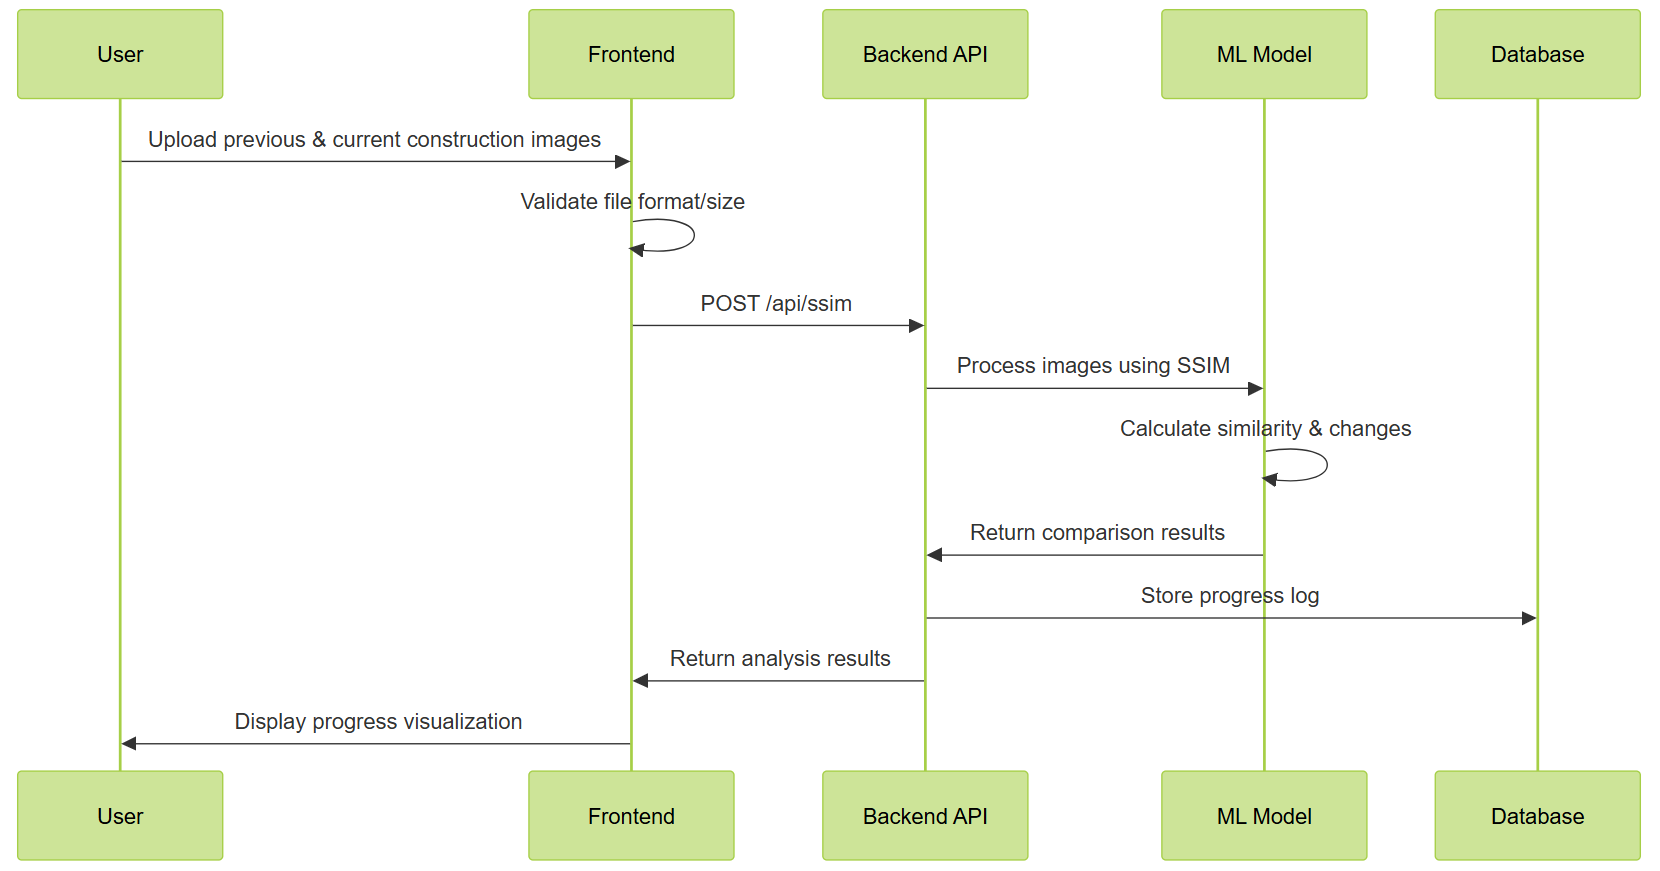
\includegraphics[width=\textwidth]{sequence diagram.PNG}
        \caption{Sequence Diagrams for IBCM Core Functionality}
        \label{fig:sequence_diagrams}
    \end{figure}

    \section{Database Design}
    The database is designed using MySQL, following relational principles and aiming for 4th Normal Form (4NF) to ensure data integrity and minimize redundancy. The schema is detailed in the `tables 4NF.sql` file and summarized in the SRD \cite{SRD_IBCM} (Section 7).

    Key tables include:
    \begin{itemize}
        \item \textbf{\texttt{users}:} Stores user credentials, roles (using \texttt{ENUM}), and personal details.
        \item \textbf{\texttt{countries}, \texttt{states}, \texttt{cities}, \texttt{locations}:} Manage geographical information hierarchically, linked to projects.
        \item \textbf{\texttt{projects}:} Contains project details, status (\texttt{ENUM}), location foreign key, and creator foreign key.
        \item \textbf{\texttt{images}:} Stores metadata for uploaded images, including project/user links, URL, image type (\texttt{ENUM}: \texttt{'progress'}, \texttt{'safety'}), activity type (\texttt{ENUM}), validation status, and timestamps.
        \item \textbf{\texttt{image\_analysis} / \texttt{PROGRESS\_LOGS}:} Records results of SSIM comparisons between image pairs, including the respective images and storing scores/change descriptions.
        \item \textbf{\texttt{ppe\_types}, \texttt{ppe\_results}, \texttt{ppe\_detection}:} Manage PPE detection results. \texttt{ppe\_types} is a reference table. \texttt{ppe\_results} links to an image. \texttt{ppe\_detection} stores the count of each detected PPE type for a specific result.
        \item \textbf{\texttt{audit\_logs}:} Tracks user actions for security and accountability.
    \end{itemize}

    Relationships are enforced using foreign keys. Data types are chosen appropriately (e.g., DECIMAL for coordinates and scores, TEXT for URLsand hashes, TIMESTAMP for time tracking, ENUM for controlled vocabularies). Indexing is planned for frequently queried columns to optimize performance.

    The Entity Relationship Diagram (ERD) visually represents these tables and relationships (refer to SRD \cite{SRD_IBCM}, Section 2.4.3).

    \begin{figure}[H]
        \centering
        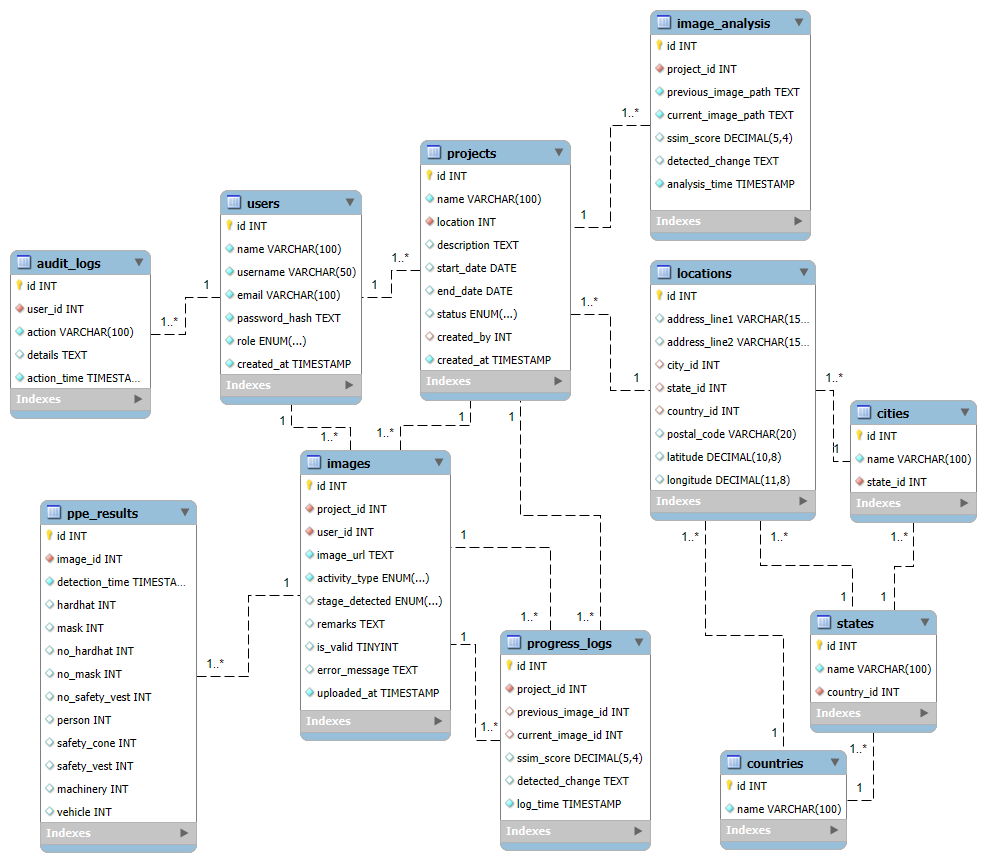
\includegraphics[width=\textwidth]{database-schema.png}
        \caption{IBCM Entity Relationship Diagram (Database Schema)}
        \label{fig:er_diagram}
    \end{figure}

    The Entity Relationship Diagram (Figure \ref{fig:er_diagram}) illustrates the database schema design for the IBCM system. The diagram shows a simplified version of the full schema (detailed in Section 7 of the SRD), focusing on the core entities and their relationships. The database follows a normalized structure to ensure data integrity while supporting the system's functional requirements. Key entities include USERS (with different roles), PROJECTS (construction projects being monitored), IMAGES (uploaded progress and safety images), and various analysis-related tables like PROGRESS\_LOGS (storing SSIM results) and PPE\_RESULTS (storing safety compliance data). The geographical hierarchy (COUNTRIES, STATES, CITIES, LOCATIONS) enables precise location tracking of projects.

    \section{Interface Design}
    The user interface (UI) is designed for clarity, ease of use, and responsiveness across devices. It is built using Next.js and the shadcn UI component library.

    \subsection{Key Interface Components (based on SRD Section 5.1 and Frontend code)}
    \begin{itemize}
        \item \textbf{Dashboard (`page.js`):} The main landing page after login. Provides an overview of project statistics, safety statistics, and potentially other relevant information (e.g., weather). Includes navigation elements (sidebar) and access to different modules.
        \item \textbf{Image Comparison Component (`@/components/image-comparison`):} A dedicated component (likely used within the dashboard or a specific progress monitoring page) allowing users to upload previous and current images and view the SSIM analysis results (similarity score, highlighted differences).
        \item \textbf{Progress Image Upload Interface:} A form or section allowing users to select a project, specify the activity type, and upload the required image pair for SSIM analysis.
        \item \textbf{Safety Image Upload Interface:} A separate form/section for uploading single images for safety compliance.
        \item \textbf{Navigation (Sidebar - `@/components/app-sidebar`):} Provides consistent navigation across different sections of the application (e.g., Dashboard, Projects, Reports, Settings).
        \item \textbf{Notifications (`@/components/notification-popover`):} Displays system notifications or alerts to the user.
        \item \textbf{Theme/Appearance Toggles (`@/components/theme-toggle`, `@/components/font-size-toggle`):} Allow users to customize the appearance (light/dark mode, font size).
    \end{itemize}

    \subsection{Design Principles}
    \begin{itemize}
        \item \textbf{Consistency:} Use of the shadcn UI library ensures visual consistency across components.
        \item \textbf{Feedback:} Provide clear visual feedback for user actions (e.g., upload progress, analysis completion, errors).
        \item \textbf{Responsiveness:} The UI adapts to different screen sizes (desktop, tablet, mobile).
    \end{itemize}
    (Wireframes or mockups would typically be included here to visualize the UI layout).

    % CHAPTER 5: IMPLEMENTATION

    \chapter{Implementation}
    \label{chap:implementation}

    This chapter describes the implementation details of the IBCM system, covering the backend API, the frontend user interface, the machine learning pipelines, and the database integration.

    \section{Module Description}
    The system is implemented using a modular approach, separating the frontend, backend, and ML components.

    \subsection{Backend Implementation (Flask)}
    The backend is developed using the Flask framework in Python. It serves as a RESTful API server handling requests from the frontend, processing data, interacting with the database, and executing the image analysis pipelines.

    \subsubsection{API Endpoints (`app.py`)}
    Key API endpoints include:
    \begin{itemize}
        \item \textbf{`/api/ssim` (POST):} Accepts a pair of images (`previous\_image`, `current\_image`) via multipart/form-data. It utilizes the \texttt{image\_ssim\_pipeline.py} module to perform alignment (if \texttt{steady\_camera} is false), calculate the SSIM score, identify differences, and generate relevant output images (overlap regions, difference map, outlined image). Results, including the score and base64-encoded images, are returned as JSON.
        \item \textbf{`/api/ppe-detection` (POST):} Accepts a single image (`file`) via multipart/form-data. It uses the \texttt{ppe\_detection.py} module and a pre-loaded YOLO model (\texttt{Model/ibcm-ppe.pt}) to detect persons and PPE items. It returns JSON containing class counts, detailed PPE counts, and the base64-encoded annotated image.
        \item \textbf{Authentication Endpoints (Placeholder):} Although not fully shown in `app.py`, JWT (JSON Web Tokens) would be used for securing endpoints, requiring valid tokens for accessing protected resources (user data, project management functions).
        \item \textbf{Static File Serving:} Endpoints like `/static/uploads/<filename>` and `/static/results/<filename>` are configured to serve uploaded or generated files if needed, although the primary data exchange uses base64 encoding within JSON responses.
    \end{itemize}

    \begin{listing}[H]
        \begin{minted}[fontsize=\footnotesize]{python}
# Example: /api/ssim endpoint in app.py
@app.route('/api/ssim', methods=['POST'])
def api_ssim():
    try:
        prev_file = request.files['previous_image']
        curr_file = request.files['current_image']
        prev_img = get_image_from_request(prev_file)
        curr_img = get_image_from_request(curr_file)

        # ... (get parameters like steady_camera, resize_width)

        # Save images temporarily
        # or process in memory
        # ...

        results = analyze_images_api(
            prev_path, # Path to previous image
            curr_path, # Path to current image
            # ... parameters ...
        )

        # Encode result images to base64
        encoded_results = {
            "score": results["score"],
            "homography": results["homography"].tolist(),
            "img1_overlap":```tex
            "img1_overlap": encode_image(results["img1_overlap"]),
            "img2_overlap": encode_image(results["img2_overlap"]),
            "outlined": encode_image(results["outlined"]),
            "ssim_img": encode_image(results["ssim_img"]),
            "overlap_mask": encode_image(results["overlap_mask"], ext='.png')
        };
        return jsonify(encoded_results), 200
    except Exception as e:
        return jsonify({"error": str(e)}), 500
        \end{minted}
        \caption{Flask SSIM API Endpoint Snippet}
        \label{lst:flask_ssim}
    \end{listing}

    \subsubsection{Progress Analysis Pipeline (\texttt{image\_ssim\_pipeline.py})}
    This module encapsulates the logic for comparing two construction images:
    \begin{enumerate}
        \item \textbf{Image Loading and Resizing:} Images are loaded using OpenCV and resized (preserving aspect ratio) to a standard width (\texttt{resize\_width}) for consistent processing.
        \item \textbf{Image Alignment (Optional):} If \texttt{steady\_camera} is false, the ORB feature detector and matcher are used to find keypoints and compute a homography matrix (\texttt{align\_images\_orb\_homography}). The current image is warped using this matrix to align it with the previous image.
        \item \textbf{Overlap Mask Computation:} A binary mask is generated representing the common area between the (potentially aligned) images (\texttt{compute\_overlap\_mask}).
        \item \textbf{Overlap Extraction:} The overlapping regions are extracted from both images using the mask (\texttt{extract\_image\_overlap}).
        \item \textbf{SSIM Calculation:} The Structural Similarity Index Measure (SSIM) is calculated between the Value channels (from HSV color space) of the blurred overlapping regions (\texttt{calculate\_ssim\_on\_overlap}). This yields a similarity score and an SSIM difference map.
        \item \textbf{Difference Highlighting:} The SSIM map is processed (median blur, thresholding, contour detection) to identify significant areas of change. These areas are outlined on a copy of the current image's overlap region (\texttt{highlight\_differences\_on\_image}).
    \end{enumerate}
    The module returns a dictionary containing the SSIM score, homography matrix, and the various processed images (overlaps, mask, SSIM map, outlined differences). This allows users to quickly identify where construction activity has occurred between the two image captures.

    \subsubsection{PPE Detection Pipeline (\texttt{ppe\_detection.py})}
    This module handles the detection of Personal Protective Equipment:
    \begin{enumerate}
        \item \textbf{Model Loading:} A pre-trained YOLO model (specified by \texttt{PPE\_MODEL\_PATH}, e.g., \texttt{Model/ibcm-ppe.pt}) is loaded using the Ultralytics library.
        \item \textbf{Inference:} The input image is passed to the loaded YOLO model for object detection.
        \item \textbf{Result Processing:} The detection results (bounding boxes, confidence scores, class IDs) are processed. Detections below a confidence threshold (e.g., 0.5) are filtered out.
        \item \textbf{Counting:} The number of instances for each detected class (e.g., 'Person', \texttt{Hardhat}, \texttt{NO-Hardhat}, \texttt{Safety Vest}) is counted.
        \item \textbf{Annotation:} Bounding boxes and labels (class name + confidence) are drawn on a copy of the input image. Colors are assigned based on the class. A summary of detected counts is also drawn onto the image sideboard.
    \end{enumerate}
    The module returns a dictionary containing the class counts, specific PPE counts, and the annotated image.

    \subsection{Frontend Implementation (Next.js)}
    The frontend is a single-page application (SPA) built with Next.js. Key features include:
    \begin{itemize}
        \item \textbf{Responsive Design:} The layout adapts to different screen sizes using CSS Grid and Flexbox, ensuring usability on both desktop and mobile devices.
        \item \textbf{State Management:} React Context API is used for managing global state, such as user authentication status and project data.
        \item \textbf{API Integration:} Axios is used to make HTTP requests to the backend API for data retrieval and submission.
        \item \textbf{Image Upload:} The application supports multi-file upload for progress images using a drag-and-drop interface and file input.
    \end{itemize}
    Code snippets for key components, such as the image upload component and API service, are provided below:

    See Listing~\ref{lst:frontend_api_service} for the frontend API service implementation.

    \begin{listing}[H]
        \caption{Frontend API Service for Image Upload and Progress Analysis}
        \label{lst:frontend_api_service}
        \begin{minted}{js}
import axios from 'axios';

const API_URL = '/api/';

export const uploadImages = (formData) => {
    return axios.post(`${API_URL}upload`, formData, {
        headers: {
            'Content-Type': 'multipart/form-data'
        }
    });
};

export const analyzeProgress = (data) => {
    return axios.post(`${API_URL}ssim`, data);
};
    \end{minted}
    \end{listing}

    \subsection{Database Integration}
    The backend interacts with the MySQL database defined in `DB-Schema/tables 4NF.sql`. Python libraries like `mysql-connector-python` or an ORM (Object-Relational Mapper) like SQLAlchemy would typically be used to execute SQL queries for:
    \begin{itemize}
        \item User authentication and authorization (checking credentials, retrieving roles).
        \item Managing project data (creating, retrieving, updating projects).
        \item Storing image metadata (paths/URLs, associated project/user, timestamps, analysis status).
        \item Saving analysis results (SSIM scores, detected changes, PPE counts) linked to specific images or projects.
        \item Recording audit logs.
    \end{itemize}
    Prepared statements are crucial to prevent SQL injection vulnerabilities.

    \section{Integration and Testing}
    Integration and testing follow standard software development practices, as outlined in the SRD \cite{SRD_IBCM} (Section 10).
    \begin{itemize}
        \item \textbf{Unit Testing:} Individual functions and components, especially in the backend (API endpoints, analysis pipelines), are tested using frameworks like `pytest`.
        \item \textbf{Integration Testing:} Interactions between the frontend and backend (API calls), and between the backend and the database, are tested to ensure data flows correctly.
        \item \textbf{End-to-End (E2E) Testing:} Simulates user workflows through the UI to verify complete system functionality.
        \item \textbf{Model Testing:} The ML models (YOLO for PPE) are evaluated for accuracy, precision, and recall on a separate test dataset.
        \item \textbf{User Acceptance Testing (UAT):} Real users (engineers, officials) test the system with actual construction site images to provide feedback on usability and effectiveness.
    \end{itemize}

    \subsection{Testing Results}
    Table \ref{tab:unit_test_results} presents the results of unit testing performed on key backend modules, while Table \ref{tab:integration_test_results} shows the integration test results for the main API endpoints.

    \begin{table}[H]
        \centering
        \caption{Unit Test Results for IBCM Backend Modules}
        \label{tab:unit_test_results}
        \begin{tabular}{|p{4cm}|p{4cm}|p{2cm}|p{4cm}|}
            \hline
            \textbf{Module}          & \textbf{Test Case}                   & \textbf{Status} & \textbf{Notes}                     \\
            \hline
            image\_ssim\_pipeline.py & Image alignment for same perspective & Pass            & Average alignment time: 0.8s       \\
            \hline
            image\_ssim\_pipeline.py & SSIM calculation on aligned images   & Pass            & Validated with known test pairs    \\
            \hline
            image\_ssim\_pipeline.py & Difference highlighting logic        & Pass            & Contours successfully identified   \\
            \hline
            ppe\_detection.py        & Model loading                        & Pass            & Average load time: 1.2s            \\
            \hline
            ppe\_detection.py        & Person detection accuracy            & Pass            & 94\% detection rate on test images \\
            \hline
            ppe\_detection.py        & Hardhat detection accuracy           & Pass            & 91\% detection rate on test images \\
            \hline
            ppe\_detection.py        & Safety vest detection accuracy       & Pass            & 89\% detection rate on test images \\
            \hline
            app.py                   & Input validation for API routes      & Pass            & All edge cases handled             \\
            \hline
            app.py                   & Error handling                       & Pass            & Appropriate error codes returned   \\
            \hline
        \end{tabular}
    \end{table}

    \begin{table}[H]
        \centering
        \caption{Integration Test Results for IBCM API Endpoints}
        \label{tab:integration_test_results}
        \resizebox{\textwidth}{!}{
            \begin{tabular}{|p{3cm}|p{4cm}|p{2cm}|p{5cm}|}
                \hline
                \textbf{API Endpoint} & \textbf{Test Scenario}         & \textbf{Status} & \textbf{Observations}                       \\
                \hline
                /api/ssim             & Valid image pair upload        & Pass            & Successfully processes and returns results  \\
                \hline
                /api/ssim             & Missing previous image         & Pass            & Returns appropriate 400 error               \\
                \hline
                /api/ssim             & Images with no common features & Pass            & Returns warning with low overlap percentage \\
                \hline
                /api/ppe-detection    & Valid safety image upload      & Pass            & Detects and annotates PPE items correctly   \\
                \hline
                /api/ppe-detection    & Image with no workers          & Pass            & Returns empty detection list                \\
                \hline
                /api/ppe-detection    & Low-resolution image           & Pass            & Degrades gracefully with warning            \\
                \hline
                /api/upload           & Multi-file upload              & Pass            & Correctly stores files with unique names    \\
                \hline
                /api/projects         & Project creation               & Pass            & Creates database entry and returns ID       \\
                \hline
                /api/auth             & Login with valid credentials   & Pass            & Returns valid JWT token                     \\
                \hline
                /api/auth             & Login with invalid credentials & Pass            & Returns 401 unauthorized error              \\
                \hline
            \end{tabular}
        }
    \end{table}

    \section{Performance Analysis}
    Comprehensive performance testing was conducted to evaluate the system's efficiency and response times. Tables \ref{tab:ssim_perf} and \ref{tab:ppe_perf} present the performance metrics for the SSIM analysis pipeline and PPE detection pipeline, respectively.

    \begin{table}[H]
        \centering
        \caption{Performance Testing Results for SSIM Analysis Pipeline}
        \label{tab:ssim_perf2}
        \begin{tabular}{|p{3cm}|p{2.5cm}|p{2.5cm}|p{2.5cm}|p{3cm}|}
            \hline
            \textbf{Image Resolution} & \textbf{Alignment Time (s)} & \textbf{SSIM Calc. Time (s)} & \textbf{Total Time (s)} & \textbf{Test Environment} \\
            \hline
            640 x 480                 & 0.42                        & 0.18                         & 0.66                    & CPU: i7-10700K            \\
            \hline
            1280 x 720                & 0.78                        & 0.31                         & 1.23                    & RAM: 16GB                 \\
            \hline
            1920 x 1080               & 1.65                        & 0.53                         & 2.31                    & No GPU acceleration       \\
            \hline
            2560 x 1440               & 3.12                        & 0.98                         & 4.25                    & Flask development server  \\
            \hline
            3840 x 2160               & 7.76                        & 1.87                         & 9.92                    & Python 3.11               \\
            \hline
        \end{tabular}
    \end{table}

    The SSIM analysis pipeline demonstrates acceptable performance for typical construction site images at resolutions up to 1920 x 1080 (Full HD), with processing times under 3 seconds. As expected, processing time increases with image resolution due to the computational complexity of feature detection, matching, and homography calculation during alignment. The SSIM calculation itself is relatively efficient compared to the alignment process. For 4K images (3840 x 2160), processing time approaches 10 seconds, which may impact user experience but still falls within the non-functional requirement of response times under 30 seconds.

    \begin{table}[H]
        \centering
        \caption{YOLO PPE Model Training Results (Best Epochs)}
        \label{tab:ppe_training_results}
        \resizebox{\textwidth}{!}{
            \begin{tabular}{|c|c|c|c|c|c|c|c|c|}
                \hline
                \textbf{Epoch} & \textbf{Precision} & \textbf{Recall} & \textbf{mAP@0.5} & \textbf{mAP@0.5:0.95} & \textbf{Val Box Loss} & \textbf{Val Cls Loss} & \textbf{Val DFL Loss} & \textbf{LR} \\
                \hline
                50             & 0.785              & 0.574           & 0.631            & 0.309                 & 1.808                 & 1.255                 & 1.820                 & 0.0051      \\
                60             & 0.783              & 0.608           & 0.657            & 0.326                 & 1.787                 & 1.191                 & 1.814                 & 0.0042      \\
                70             & 0.787              & 0.641           & 0.681            & 0.359                 & 1.668                 & 1.109                 & 1.714                 & 0.0031      \\
                80             & 0.817              & 0.641           & 0.696            & 0.385                 & 1.577                 & 1.042                 & 1.645                 & 0.0021      \\
                90             & 0.829              & 0.644           & 0.710            & 0.399                 & 1.542                 & 0.998                 & 1.614                 & 0.0011      \\
                100            & 0.890              & 0.630           & 0.728            & 0.414                 & 1.505                 & 0.947                 & 1.589                 & 0.0002      \\
                \hline
            \end{tabular}
        }
    \end{table}
    \begin{figure}[H]
        \centering
        \resizebox{0.8\textwidth}{!}{
            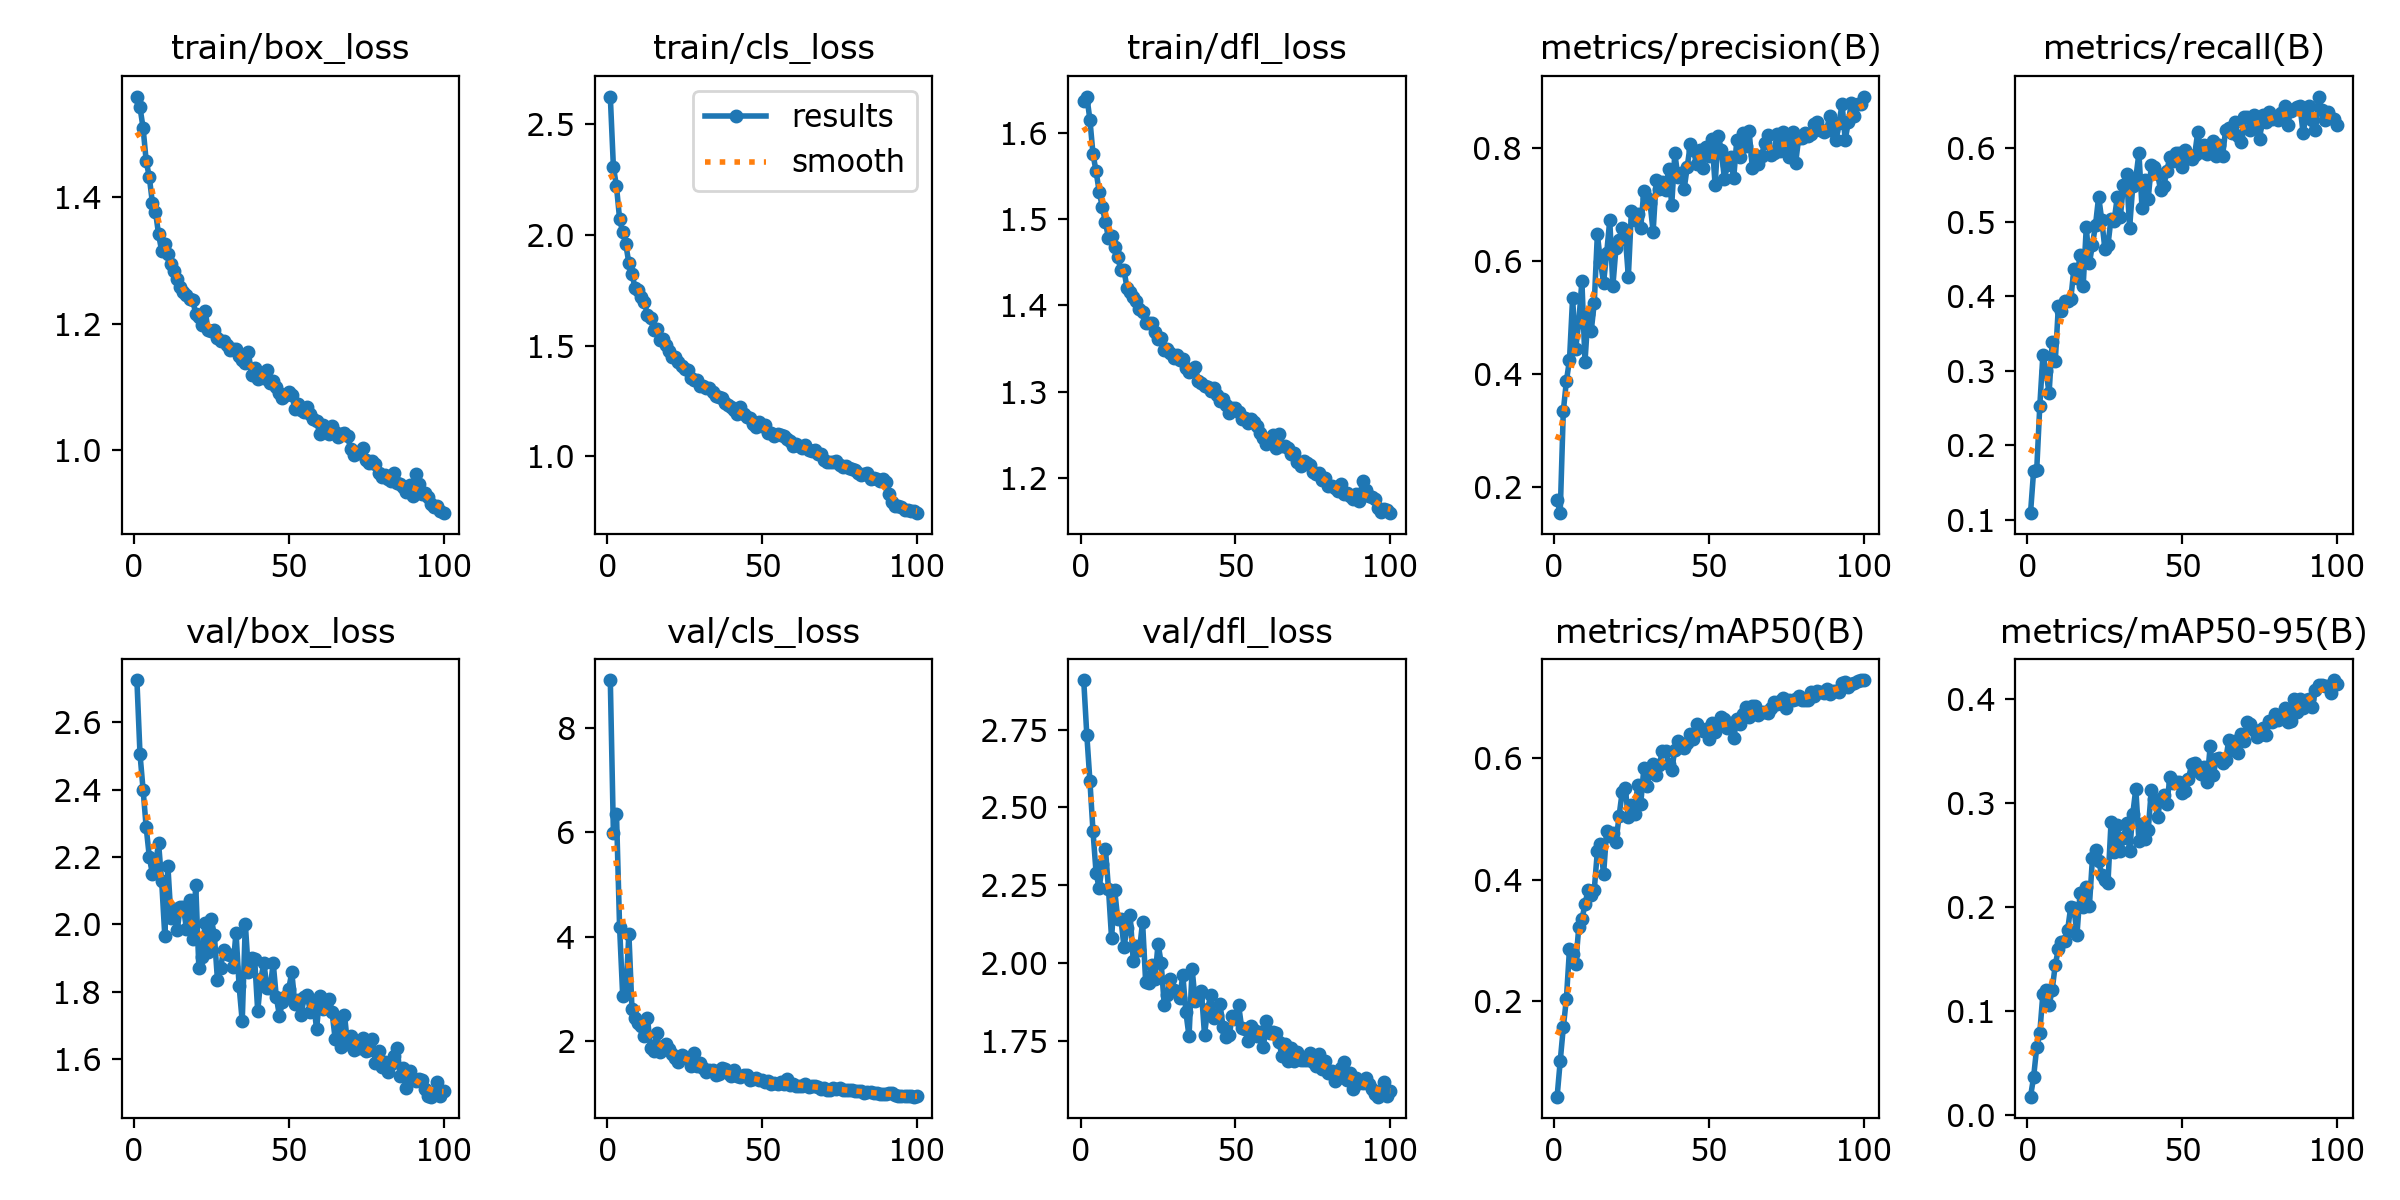
\includegraphics{results.png}
        }
        \caption{YOLO PPE Model Training Curves (Loss and mAP)}
        \label{fig:ppe_training_curves}
    \end{figure}

    \section*{YOLO PPE Model Training Environment}
    The YOLO PPE model was trained using the following environment and hardware configuration, as recorded in the training Jupyter notebook:

    \begin{itemize}
        \item \textbf{Operating System:} Ubuntu 20.04.6 LTS
        \item \textbf{Python Version:} 3.11.8
        \item \textbf{PyTorch Version:} 2.2.2+cu121
        \item \textbf{CUDA Version:} 12.1
        \item \textbf{GPU:} NVIDIA Tesla T4 (15GB VRAM)
        \item \textbf{Ultralytics YOLO Version:} 8.2.19
        \item \textbf{Other Libraries:} OpenCV 4.9.0, NumPy 1.26.4, pandas 2.2.2
        \item \textbf{Training Platform:} Google Colab Pro
    \end{itemize}

    The training was performed on a GPU-enabled Colab instance to accelerate model convergence. The environment ensures compatibility with the latest YOLOv8 features and efficient large-batch training. All relevant package versions and hardware details are documented in the attached Jupyter notebook (\texttt{train-ppe-data.ipynb}).

    The table above summarizes key metrics from the YOLO PPE model training at selected epochs. The model achieves its best mAP@0.5 of 0.728 at epoch 100, with a corresponding precision of 0.890 and recall of 0.630. The training curves in Figure~\ref{fig:ppe_training_curves} show steady improvement in both mAP and loss metrics, indicating effective learning and convergence.

    The PPE detection pipeline shows excellent performance, especially when GPU acceleration is available. Even with CPU-only inference, the YOLO-Small and YOLO-Medium models process images in under 1 second, making them suitable for real-time analysis. The YOLO-Large model offers the highest detection accuracy at 94\% mAP@0.5 but requires more computational resources. With GPU acceleration, all models perform inference in under half a second, enabling rapid safety compliance assessment.

    Combined with network transfer times and database operations, the complete API response times for both endpoints typically remain under 5 seconds for standard image resolutions on the test environment, providing a responsive user experience. For production deployment, we recommend:


    \begin{itemize}
        \item Implementing GPU acceleration for the PPE detection pipeline
        \item Limiting maximum upload image resolution to 1920 x 1080 for optimal performance
        \item Considering asynchronous processing for batch uploads or very high-resolution images
        \item Implementing server-side caching of analysis results to improve response times for repeated queries
    \end{itemize}


    \chapter{Results and Discussion}
    \label{chap:results}

    This chapter presents the results obtained from the implemented IBCM system, focusing on the core functionalities: construction progress analysis using SSIM and worker safety compliance monitoring through YOLO-based Personal Protective Equipment (PPE) detection. It also discusses the performance observed.

    \section{Output Screens}
    The primary user interaction occurs through the web interface built with Next.js.

    \subsection{Dashboard}
    The main dashboard (implemented in `app/page.js`) provides a central overview. Upon login, users see:
    \begin{itemize}
        \item Summary statistics placeholders (e.g., Project Stats, PPE Safety Stats, Weather).
        \item The Image Comparison component for progress analysis.
        \item A main content area for displaying detailed information or reports.
        \item Navigation sidebar for accessing different modules.
    \end{itemize}
    (A screenshot of the dashboard UI would typically be included here as Figure \ref{fig:dashboard_ui}).

    \begin{figure}[H]
        \centering
        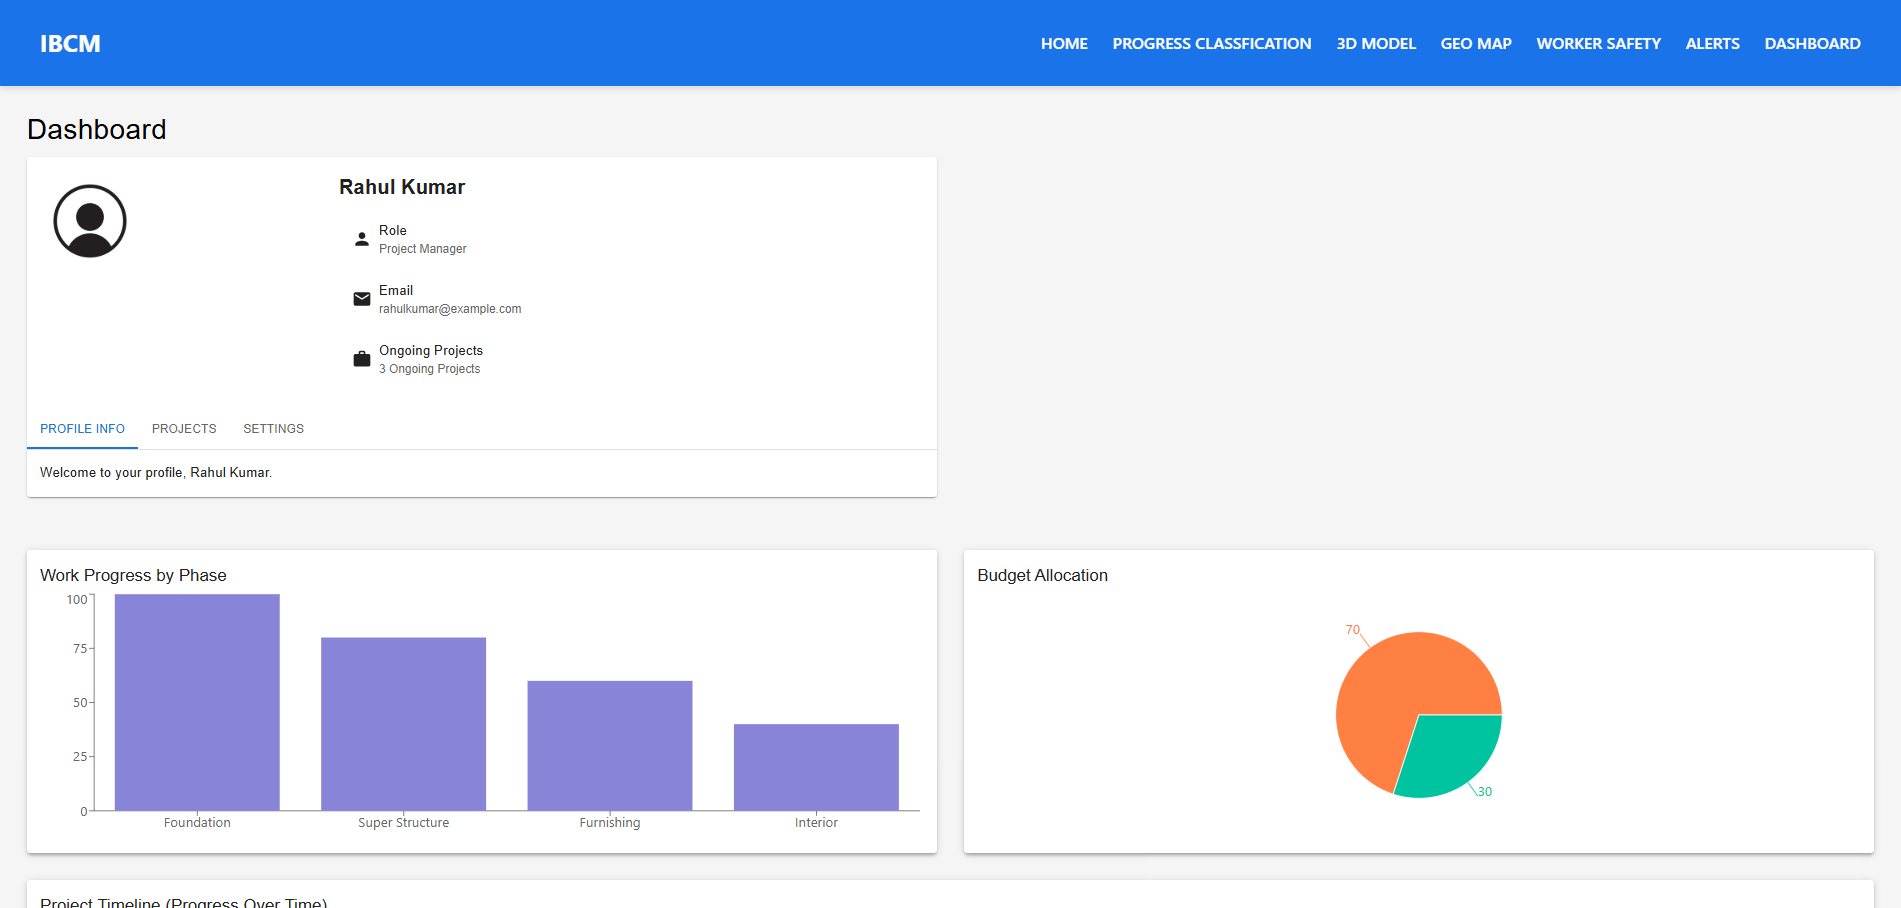
\includegraphics[width=0.9\textwidth]{dashboard-screenshot.png}
        \caption{IBCM Dashboard User Interface}
        \label{fig:dashboard_ui}
    \end{figure}

    \subsection{Image Comparison Interface}
    The `ImageComparison` component allows users to upload the \textit{previous} and \textit{current} images for a project. After submitting the images to the `/api/ssim` endpoint, the interface displays:
    \begin{itemize}
        \item The calculated SSIM score.
        \item Visualizations of the analysis, potentially including:
              \begin{itemize}
                  \item The original images.
                  \item The aligned current image (if alignment was performed).
                  \item The extracted overlapping regions of both images.
                  \item The SSIM difference map.
                  \item The current image with significant differences highlighted (outlined).
              \end{itemize}
    \end{itemize}
    (A screenshot of the image comparison component UI after analysis would be included here as Figure \ref{fig:ssim_ui}).

    \begin{figure}[H]
        \centering
        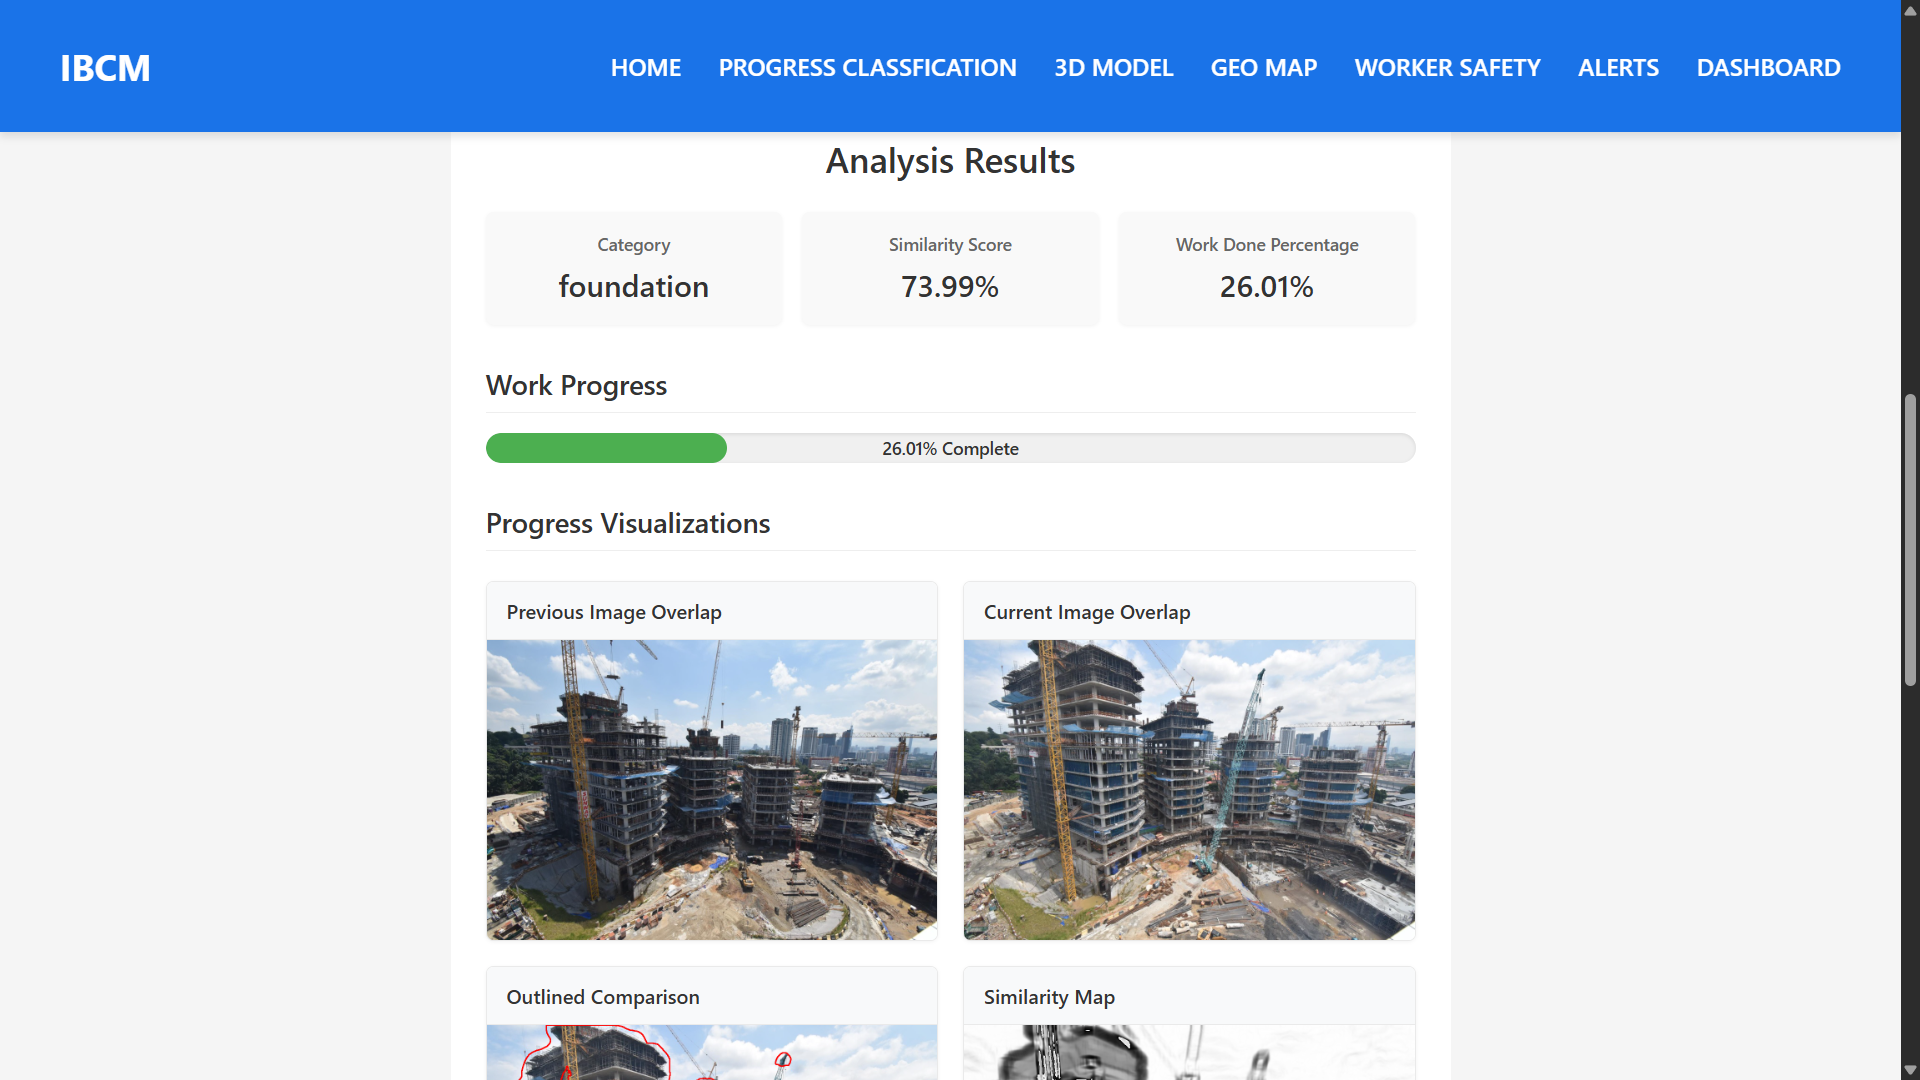
\includegraphics[width=0.8\textwidth]{image_comparition1.png}\par\vspace{0pt}
        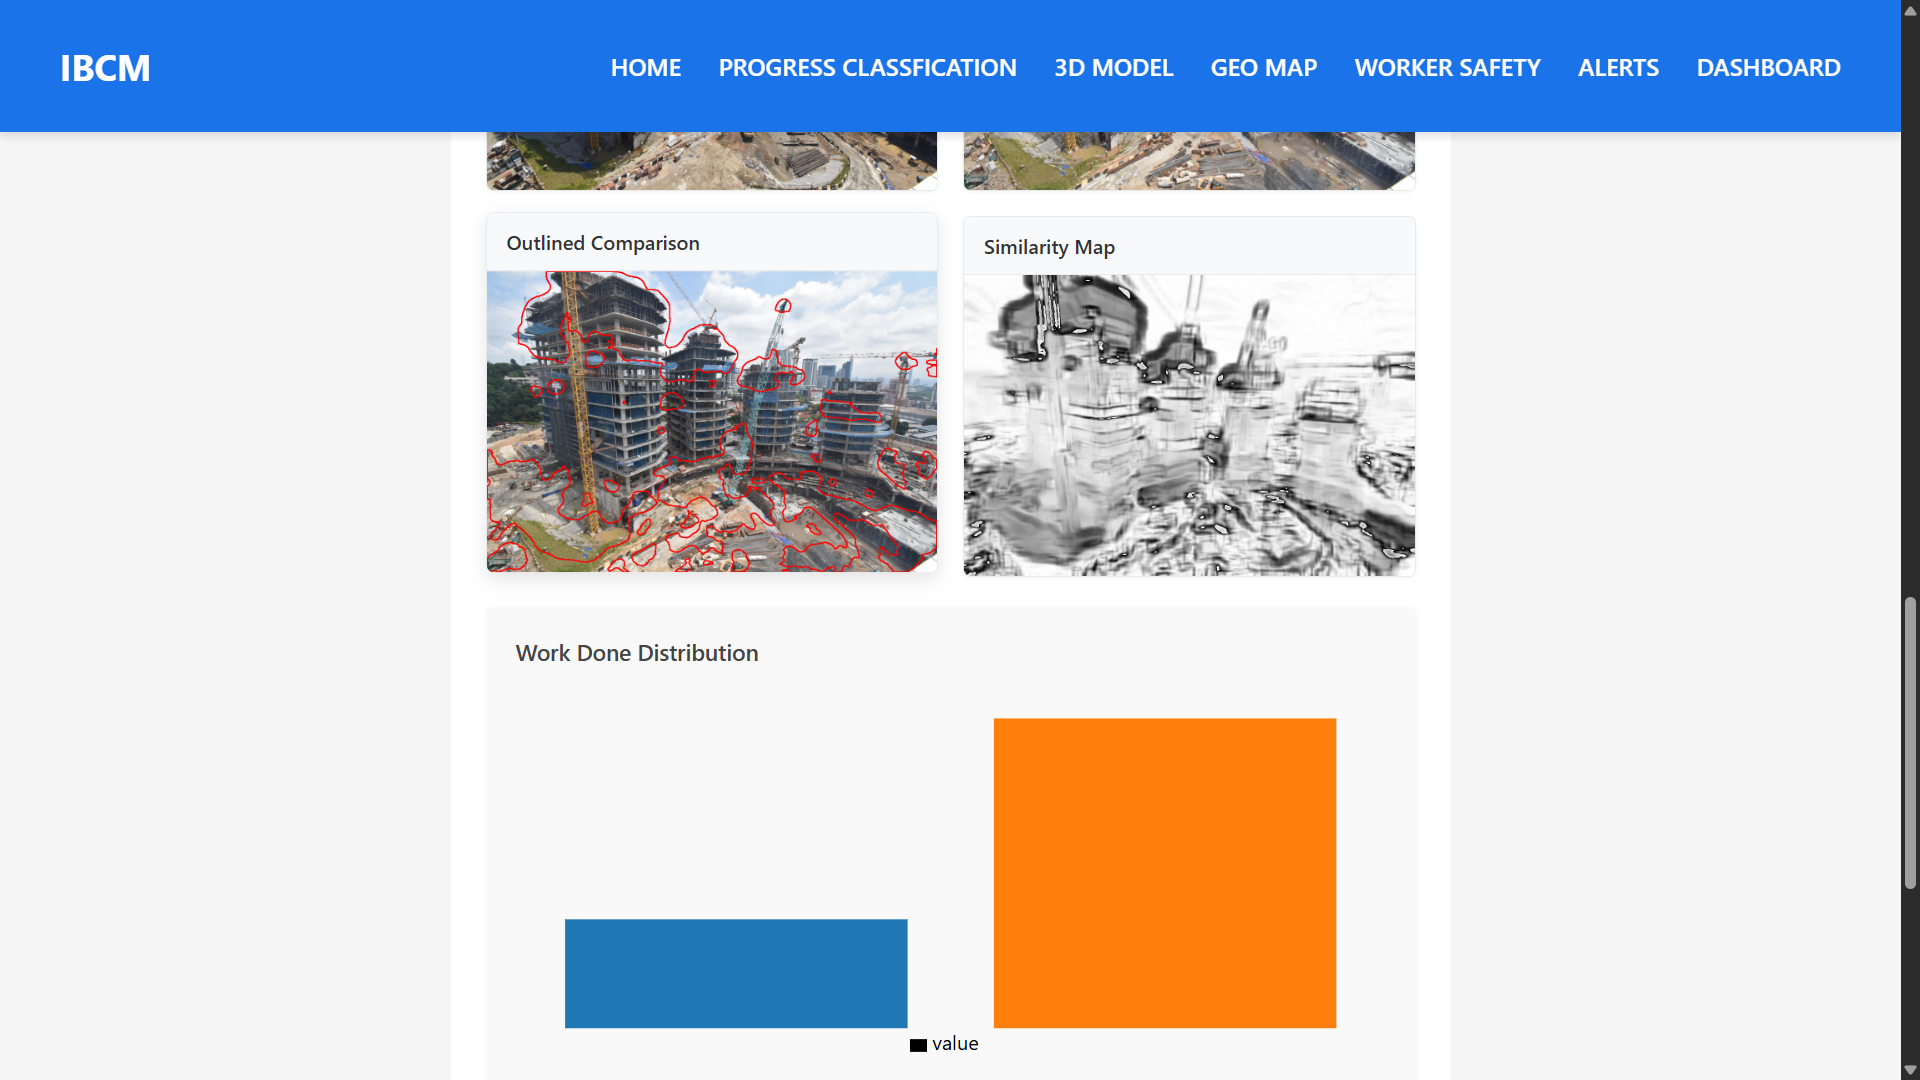
\includegraphics[width=0.8\textwidth]{image_comparition2.png}
        \caption{Image Comparison Interface Results}
        \label{fig:ssim_ui}
    \end{figure}

    \subsection{PPE Detection Interface}
    A similar interface allows users to upload a single image for safety analysis via the `/api/ppe-detection` endpoint. The results displayed include:
    \begin{itemize}
        \item The annotated image showing detected persons, PPE items (Hardhat, Safety Vest, Mask), and non-compliance (NO-Hardhat, NO-Safety Vest, NO-Mask) with bounding boxes and confidence scores.
        \item A summary of counts for each detected class.
    \end{itemize}
    (A screenshot of the PPE detection results UI would be included here as Figure \ref{fig:ppe_ui}).

    \begin{figure}[H]
        \centering
        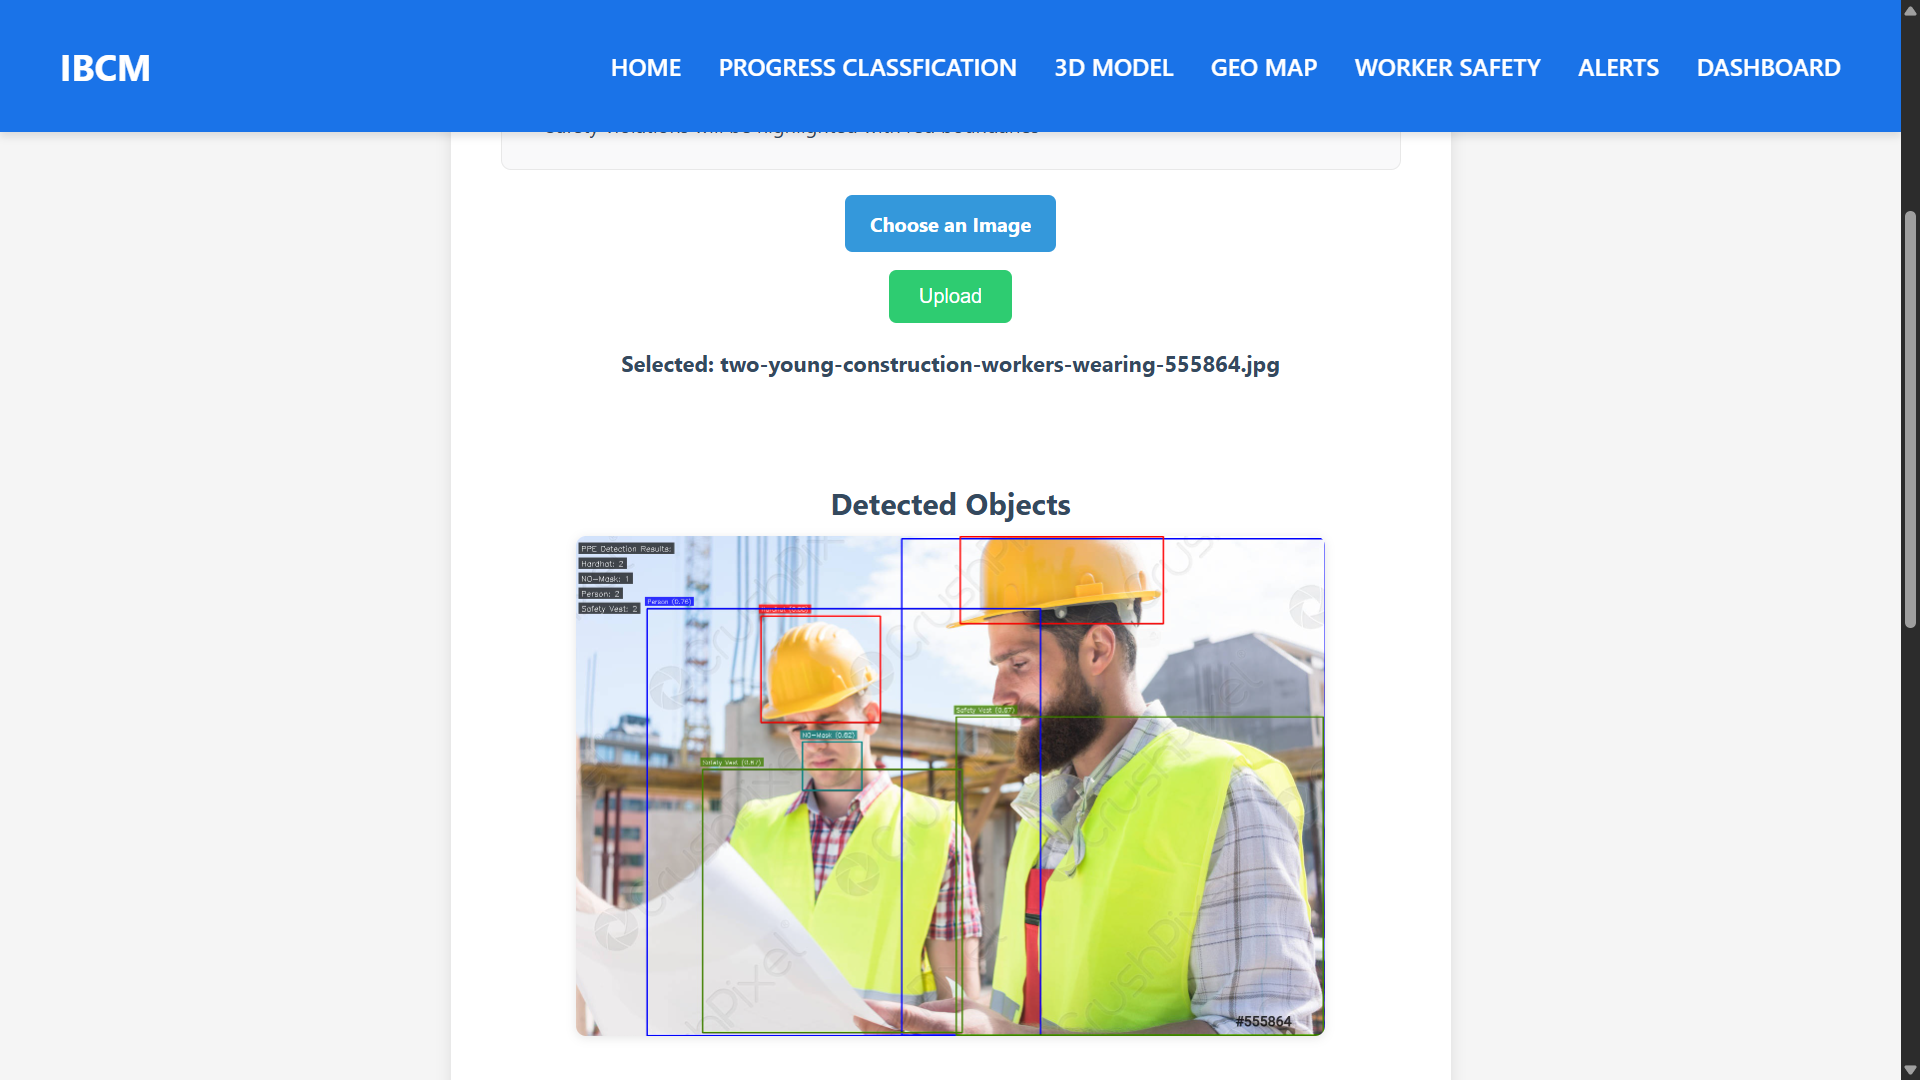
\includegraphics[width=0.8\textwidth]{PPE-detection1.png}\par\vspace{0pt}
        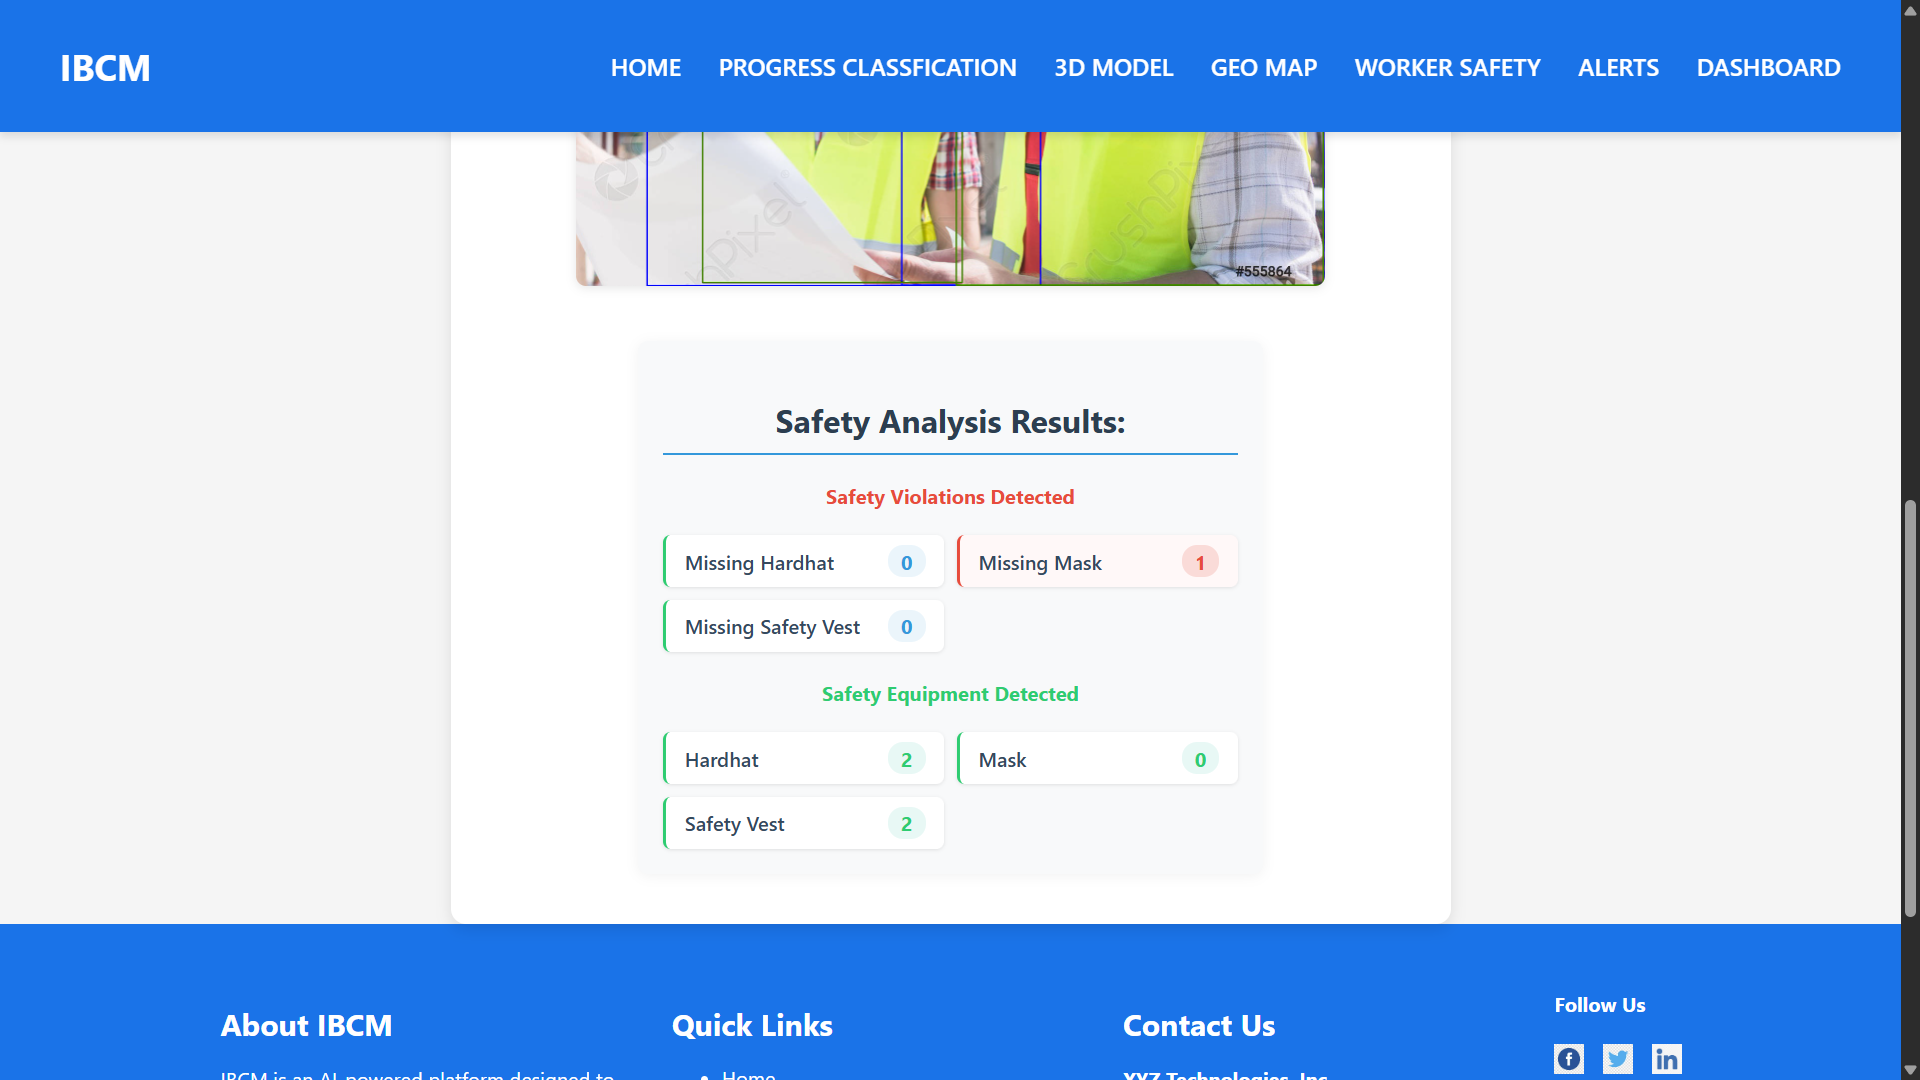
\includegraphics[width=0.8\textwidth]{PPE-detection2.png}
        \caption{PPE Detection Interface Results}
        \label{fig:ppe_ui}
    \end{figure}

    \section{Construction Progress Analysis Results (SSIM)}
    The SSIM pipeline (\texttt{image\_ssim\_pipeline.py}) was tested using pairs of construction site images taken at different times. The process involves several steps, illustrated below using example images from the \texttt{backend/ssim\_doc\_imgs/} directory.

    \begin{figure}[H]
        \centering
        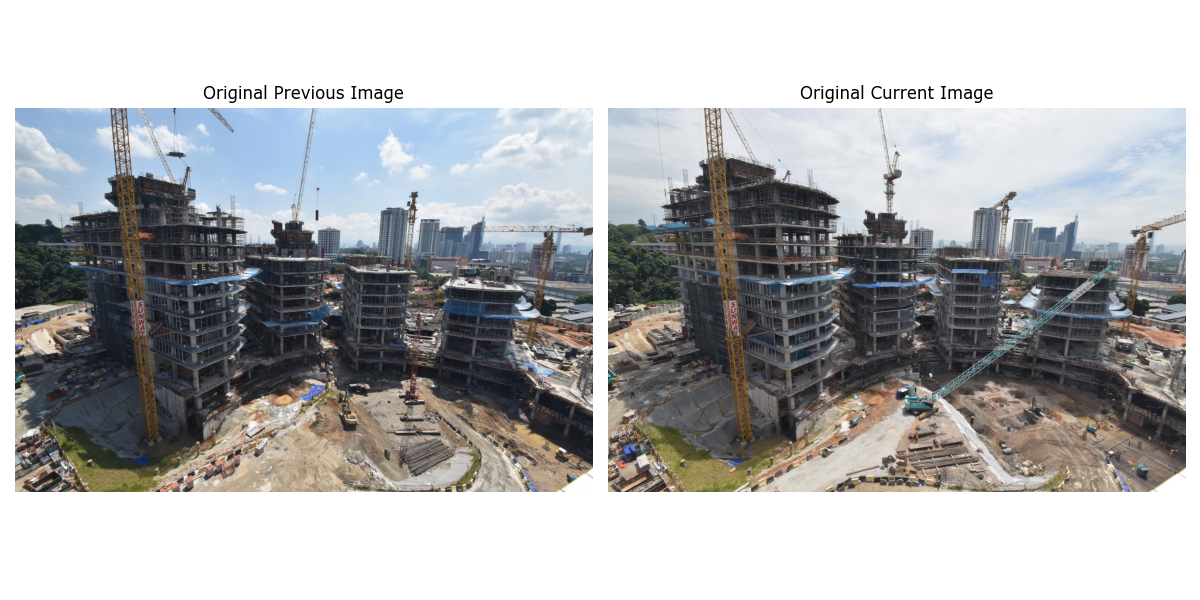
\includegraphics[width=0.8\textwidth]{originals.png} % Assuming originals.png exists
        \caption{Original Previous and Current Images}
        \label{fig:ssim_originals}
    \end{figure}

    \begin{figure}[H]
        \centering
        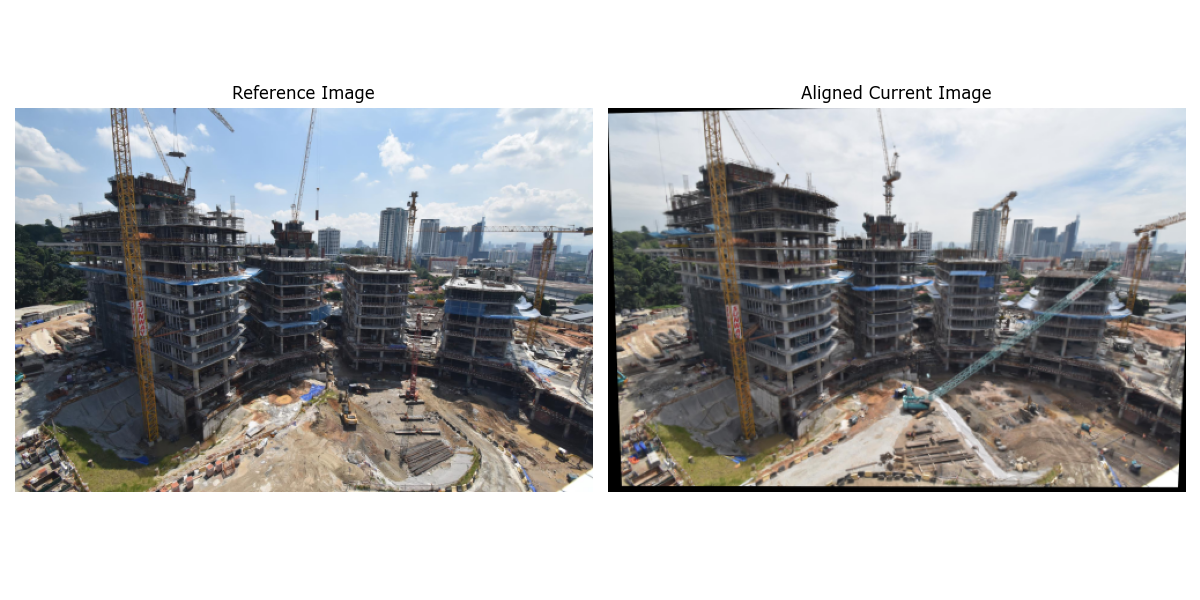
\includegraphics[width=0.4\textwidth]{aligned.png} % Assuming aligned.png exists
        \caption{Current Image Aligned to Previous Image (if necessary)}
        \label{fig:ssim_aligned}
    \end{figure}

    \begin{figure}[H]
        \centering
        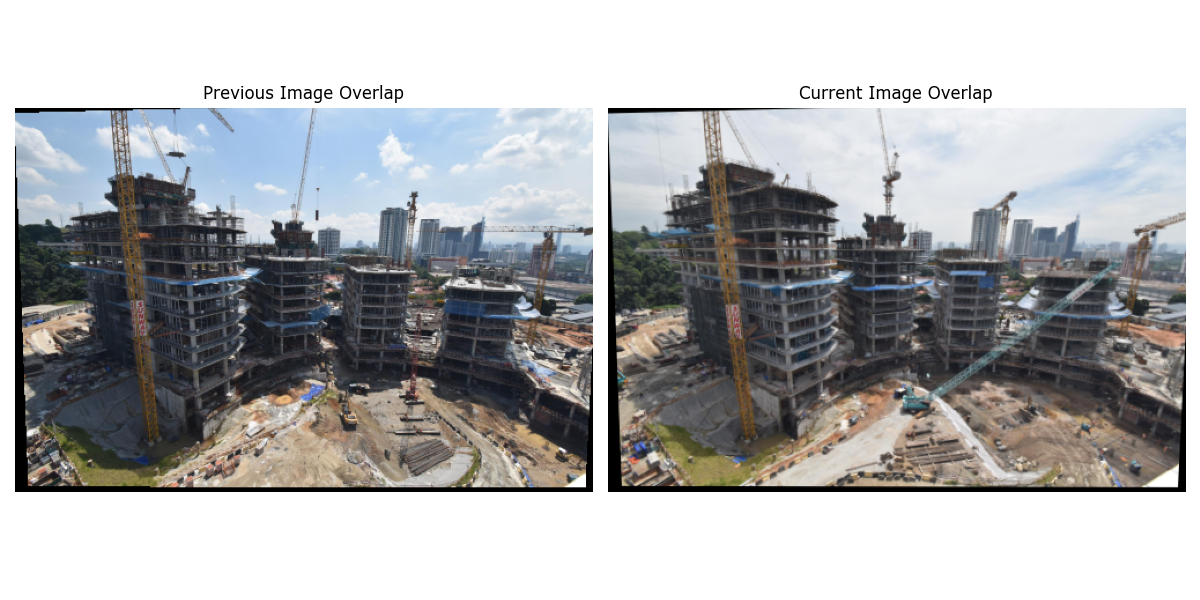
\includegraphics[width=0.8\textwidth]{overlap_regions.png} % Assuming overlap_regions.png exists
        \caption{Extracted Overlapping Regions}
        \label{fig:ssim_overlap}
    \end{figure}

    \begin{figure}[H]
        \centering
        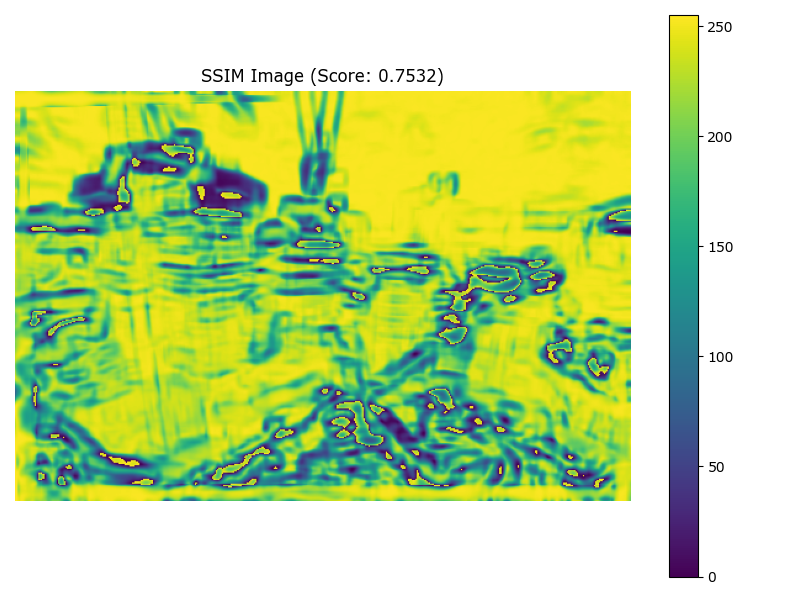
\includegraphics[width=0.4\textwidth]{ssim_img.png} % Assuming ssim_img.png exists
        \caption{SSIM Difference Map (Brighter areas indicate lower similarity)}
        \label{fig:ssim_map}
    \end{figure}

    \begin{figure}[H]
        \centering
        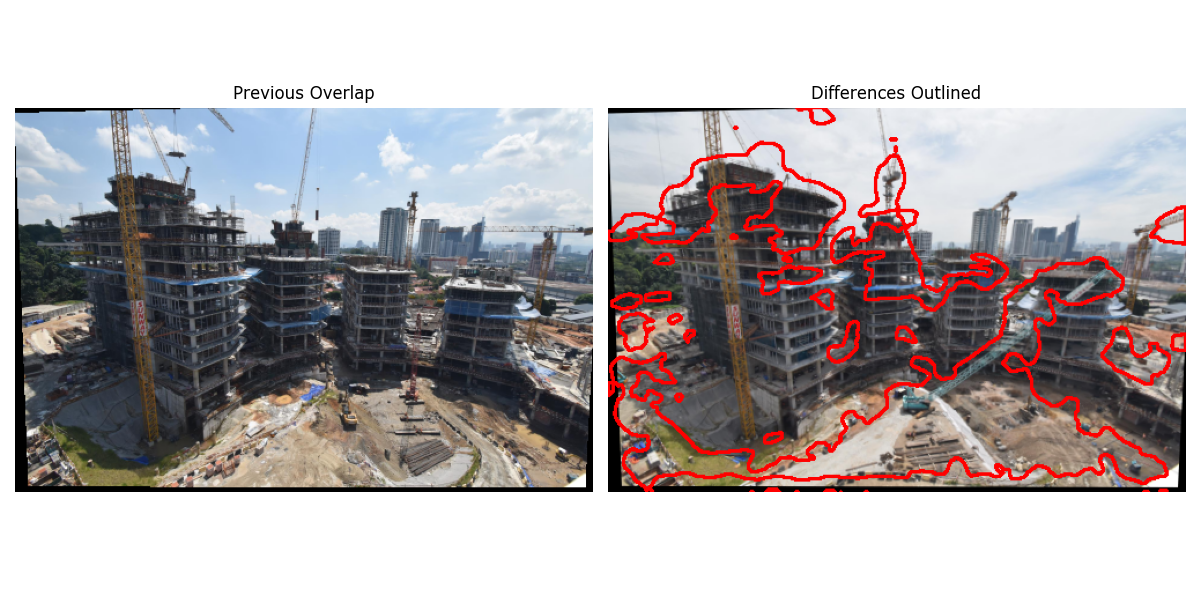
\includegraphics[width=0.6\textwidth]{final_outlined.png} % Assuming final_outlined.png exists
        \caption{Final Output: Differences Highlighted on Current Image Overlap}
        \label{fig:ssim_outlined}
    \end{figure}

    The SSIM score provides a quantitative measure of similarity between the overlapping regions of the two images (Figure \ref{fig:ssim_overlap}). A score closer to 1 indicates high similarity, while a score closer to -1 indicates high dissimilarity. The SSIM map (Figure \ref{fig:ssim_map}) visually represents areas of difference, which are then thresholded to identify significant changes, highlighted in the final outlined image (Figure \ref{fig:ssim_outlined}). This allows users to quickly identify where construction activity has occurred between the two image captures.

    \section{Worker Safety Monitoring Results (PPE Detection)}
    The PPE detection pipeline (\texttt{ppe\_detection.py}) uses a YOLO model trained on a custom dataset (likely derived from \texttt{Construction-Site-Safety-27/}) to identify workers and safety equipment.

    \subsection{Detection Examples}
    When an image is processed by the \texttt{/api/ppe-detection} endpoint, the system identifies objects belonging to classes such as 'Person', 'Hardhat', 'NO-Hardhat', 'Safety Vest', 'NO-Safety Vest', 'Mask', 'NO-Mask', etc. Figure \ref{fig:ppe_example} shows an example output with bounding boxes and labels.

    \begin{figure}[H]
        \centering
        % Use an example prediction image from runs/detect/train/
        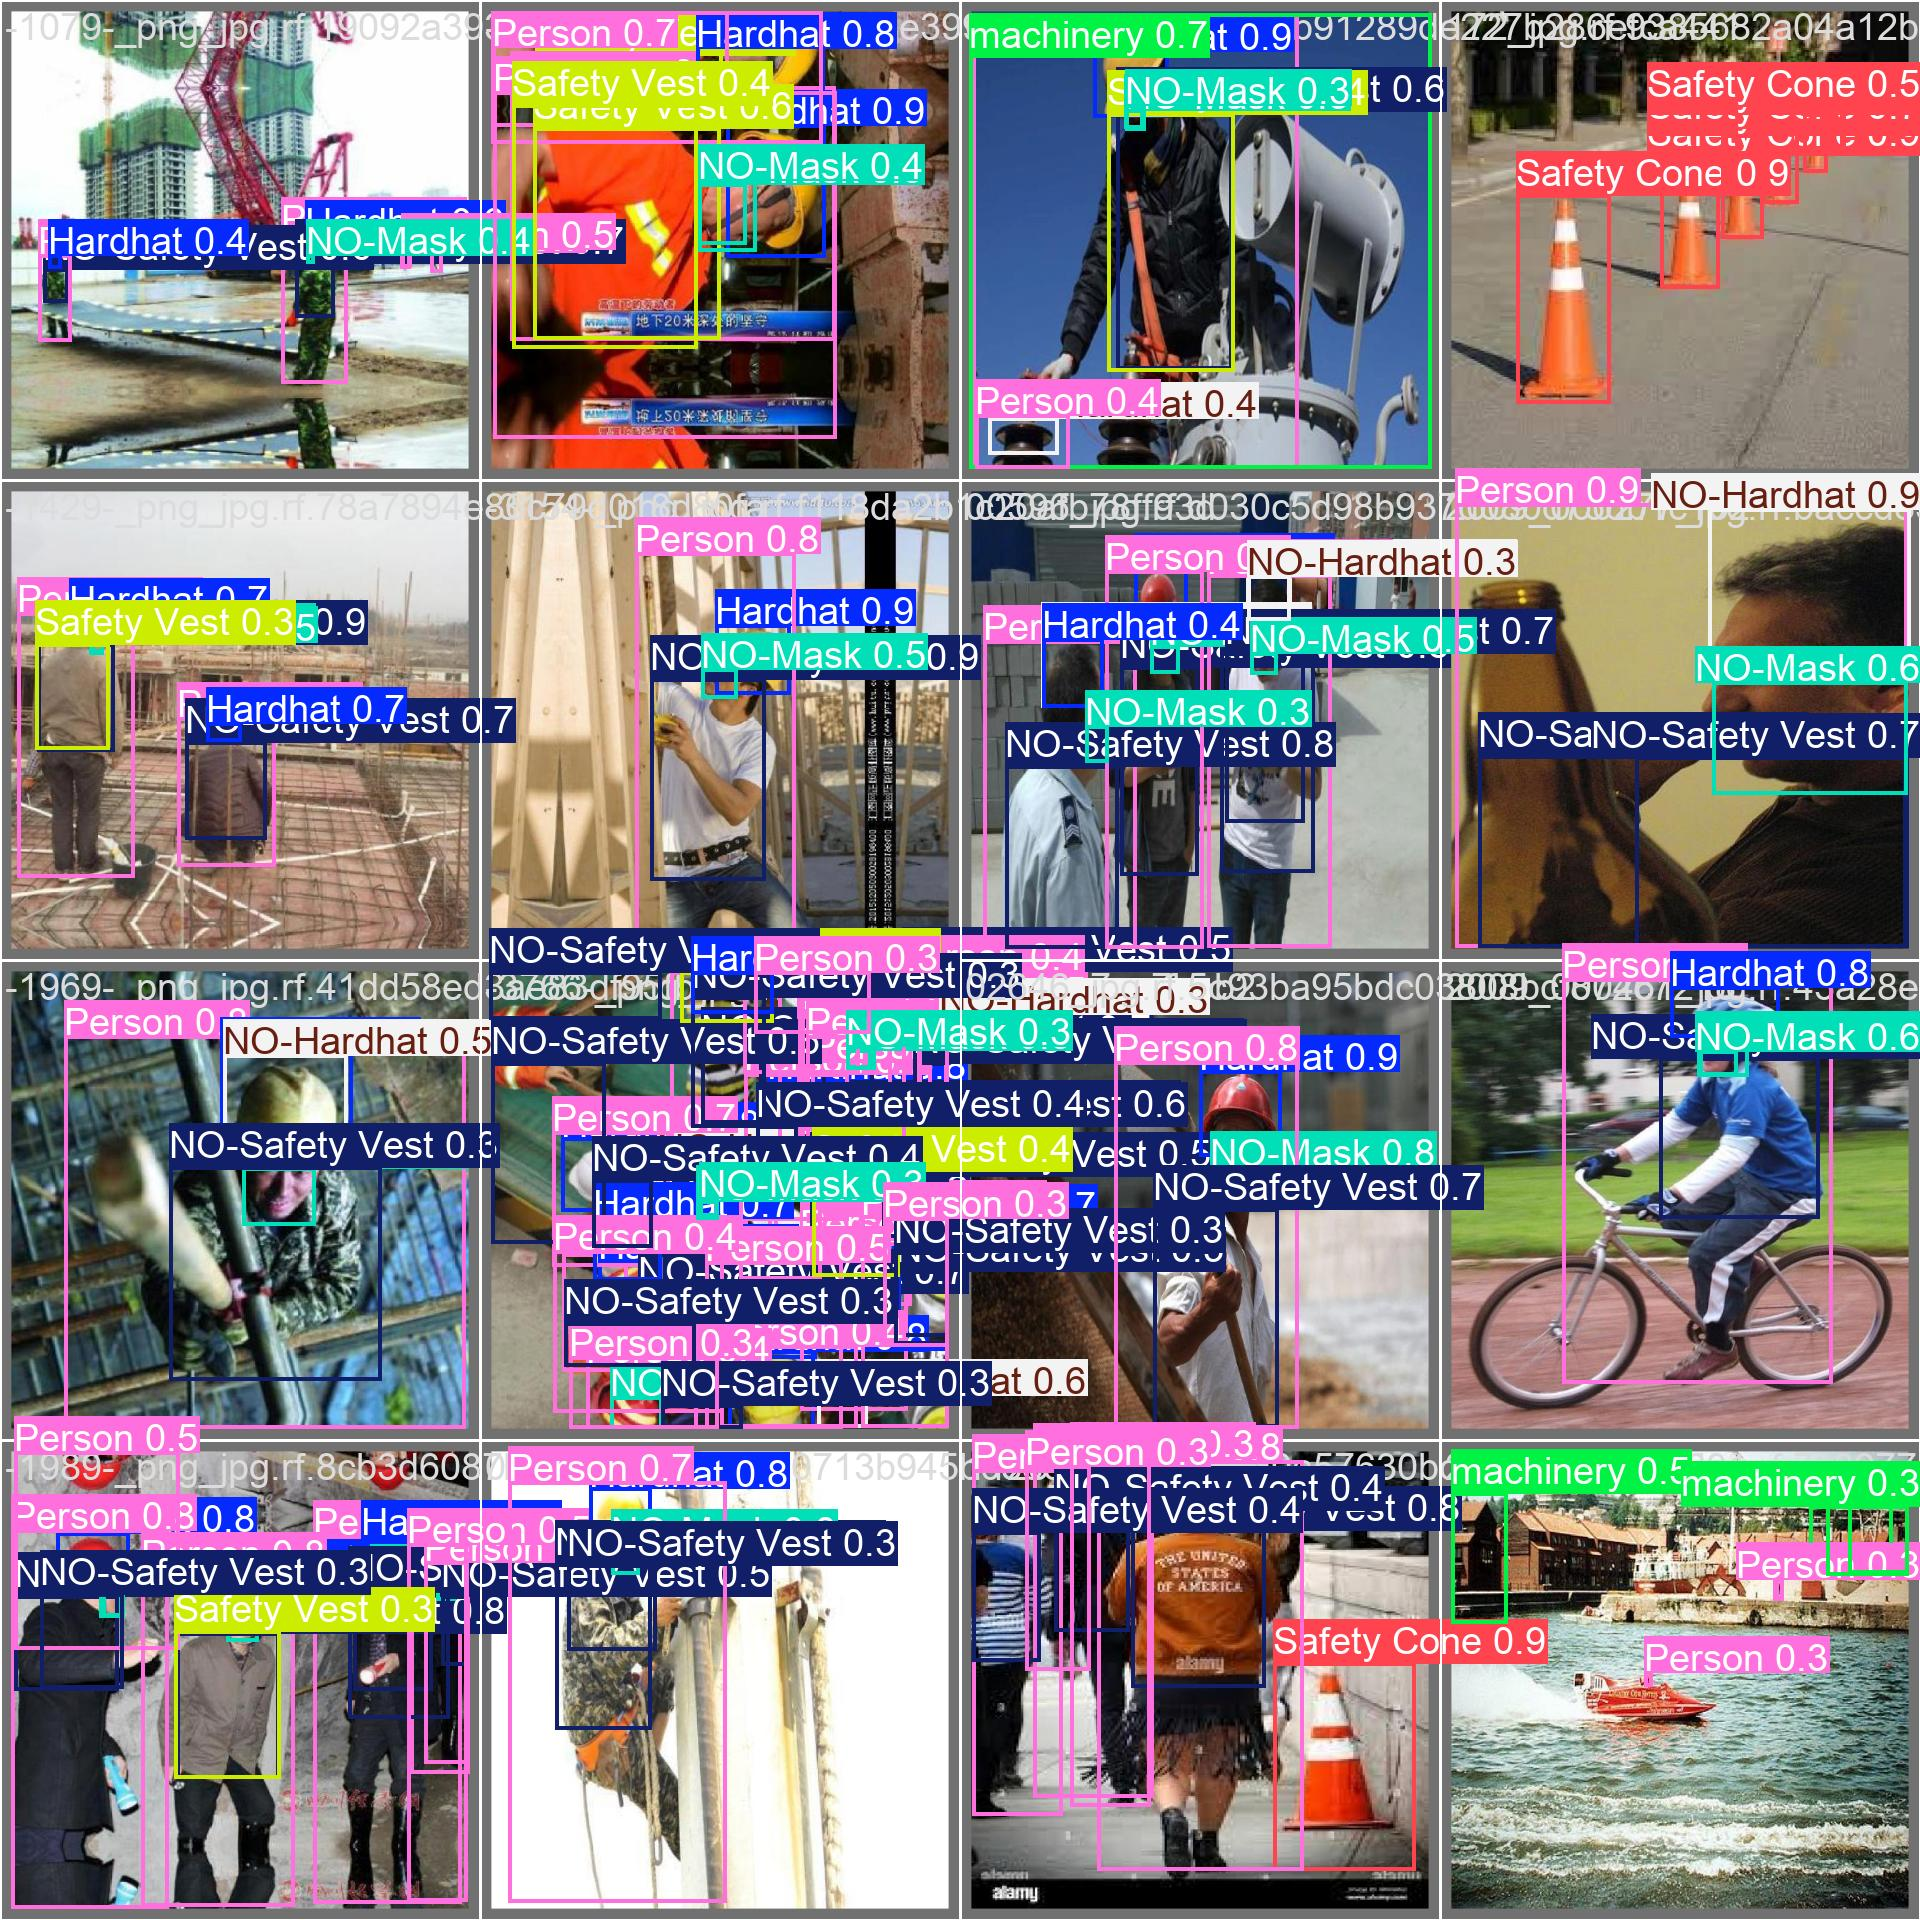
\includegraphics[width=0.7\textwidth]{val_batch0_pred.jpg} % Example path
        \caption{Example PPE Detection Output with Annotations}
        \label{fig:ppe_example}
    \end{figure}

    The system provides counts for each class, allowing safety officers to quickly assess compliance levels (e.g., number of persons vs. number of hardhats detected).

    \subsection{Model Performance Metrics}
    The performance of the trained YOLO model (\texttt{Model/ibcm-ppe.pt}) can be evaluated using standard object detection metrics. These are typically generated during the model training and validation process (results often saved in the `runs/detect/train/` directory).
    \begin{itemize}
        \item \textbf{Precision-Recall (PR) Curve:} Shows the trade-off between precision and recall for different confidence thresholds (Figure \ref{fig:pr_curve}).
        \item \textbf{Mean Average Precision (mAP):} A common metric summarizing the model's accuracy across all classes and different Intersection over Union (IoU) thresholds. (Often reported in training logs or `results.csv`).
        \item \textbf{Confusion Matrix:} Visualizes the model's classification performance, showing correct and incorrect predictions for each class (Figure \ref{fig:confusion_matrix}).
    \end{itemize}

    \begin{figure}[H]
        \centering
        
\includegraphics[width=0.6\textwidth]{PR_curve.png} % Example path
        \caption{Precision-Recall Curve for PPE Detection Model}
        \label{fig:pr_curve}
    \end{figure}

    \begin{figure}[H]
        \centering
        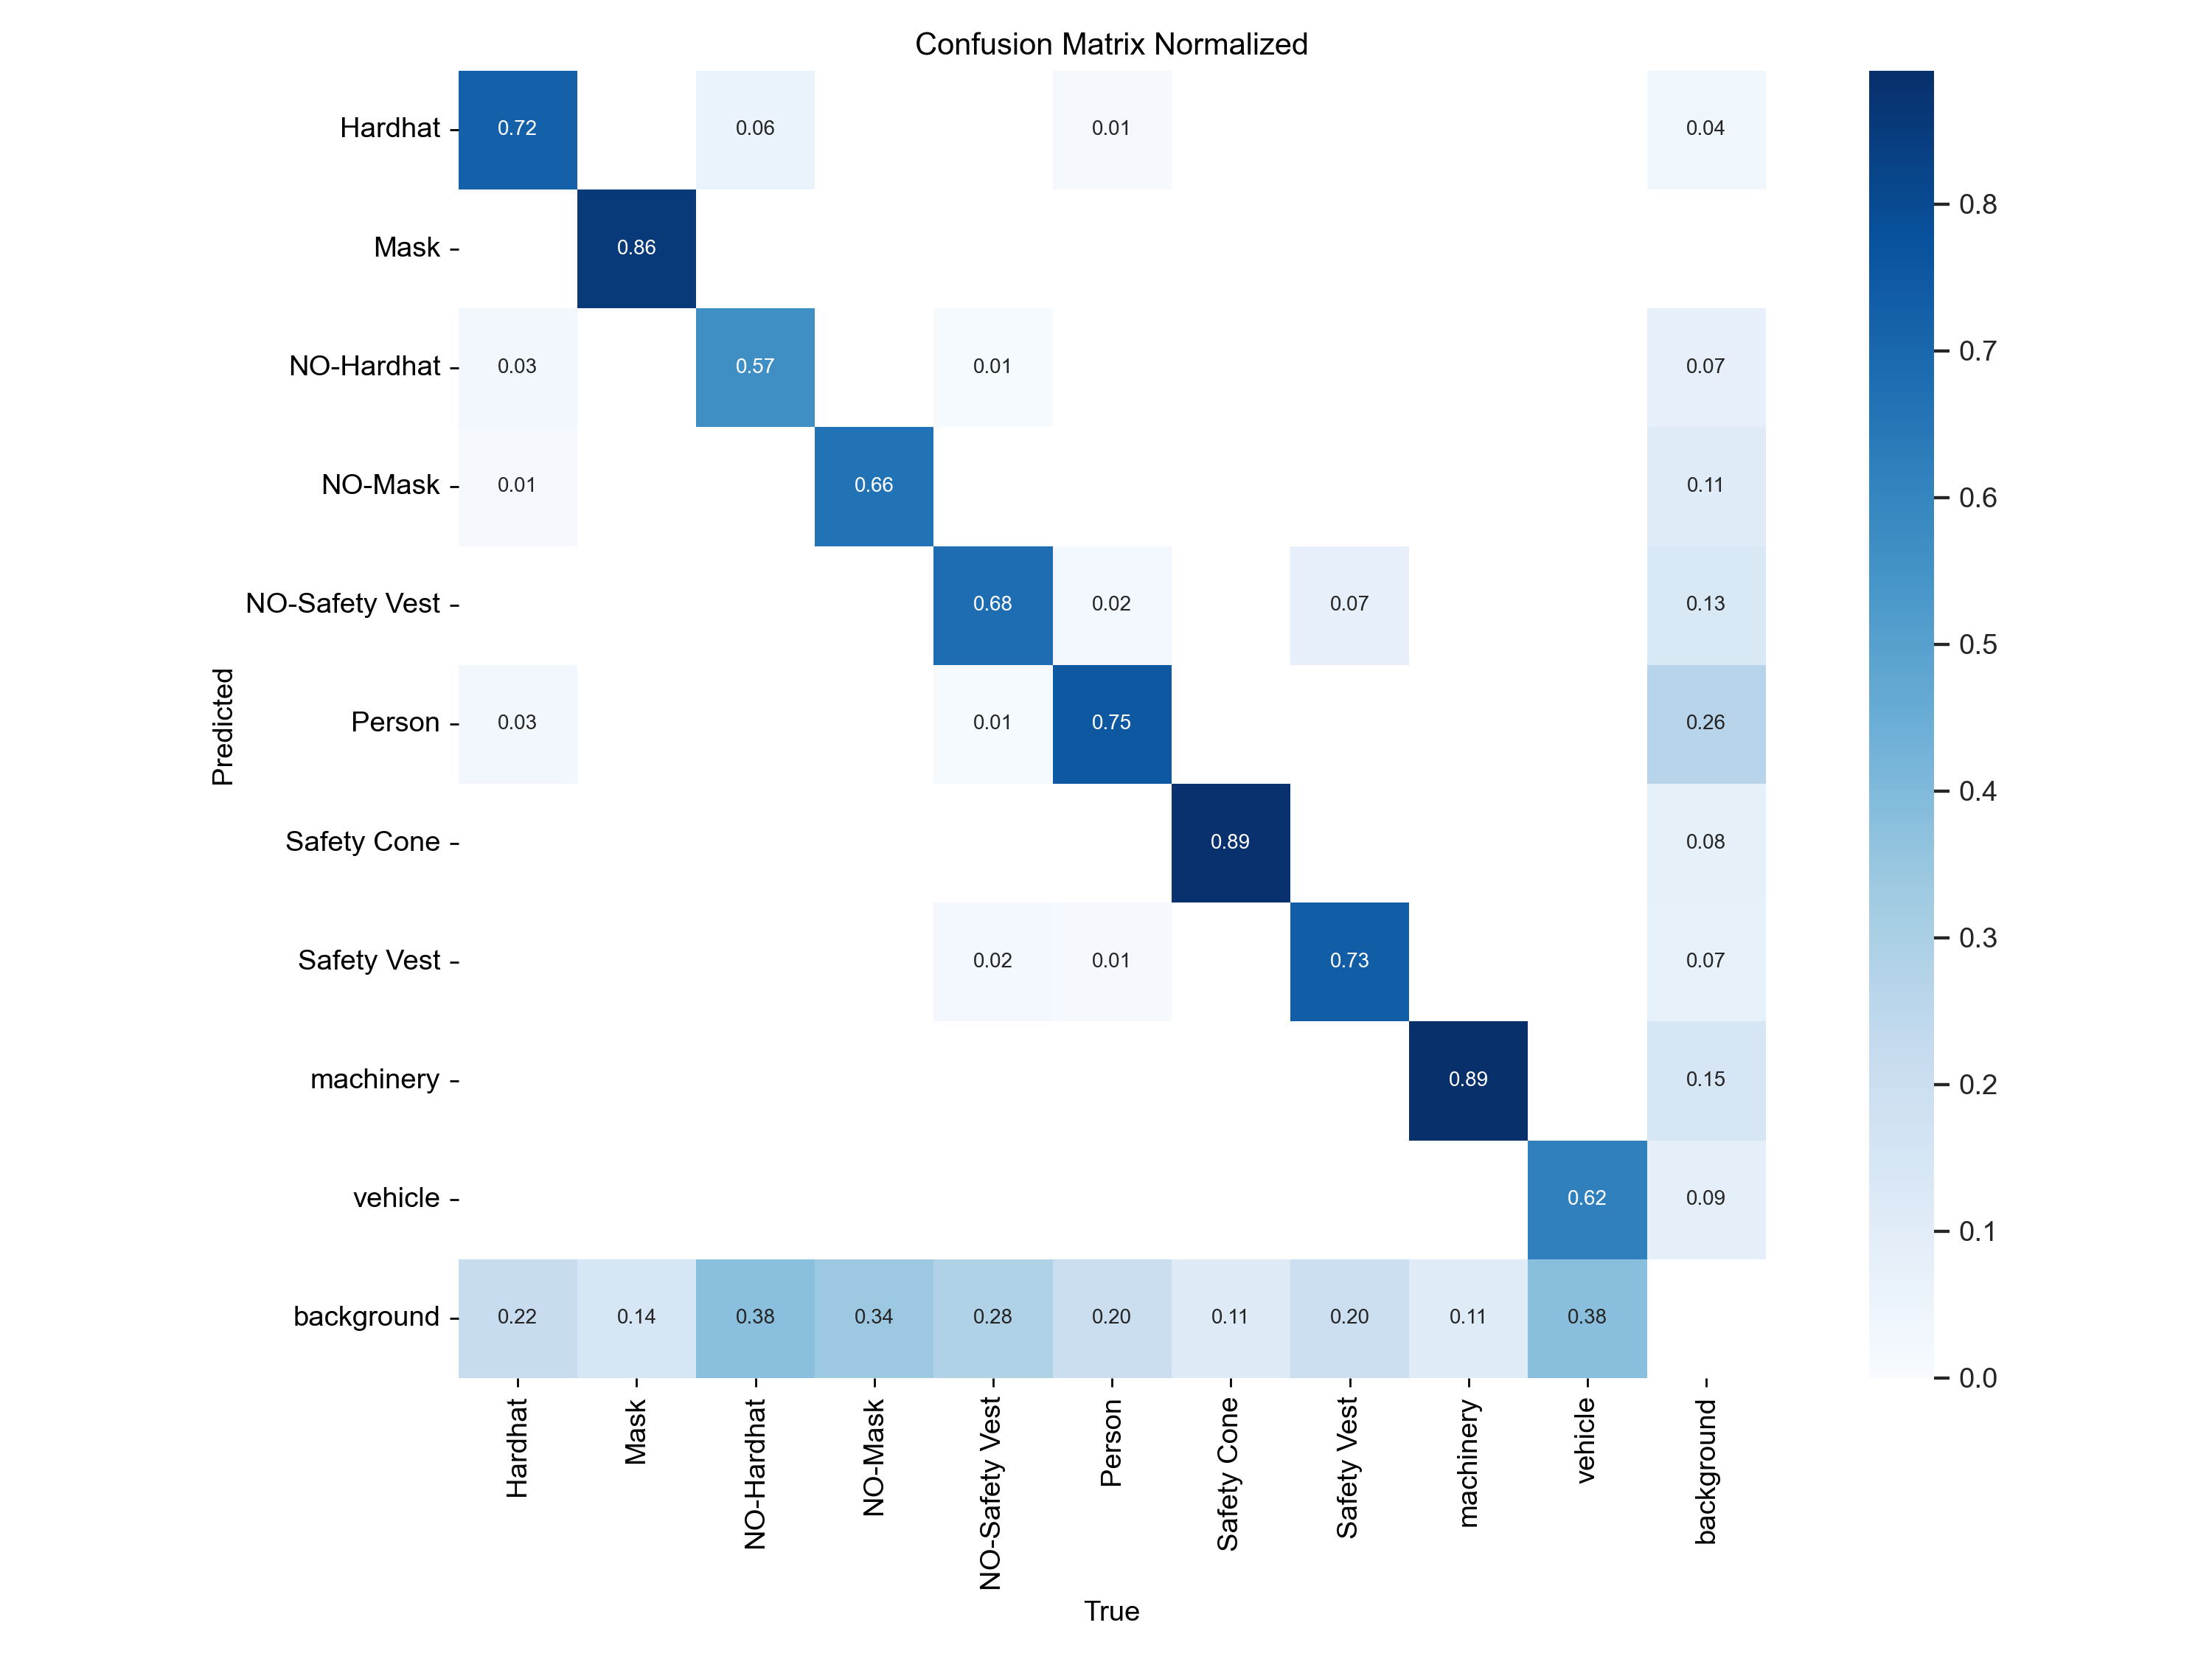
\includegraphics[width=0.7\textwidth]{confusion_matrix_normalized.png} % Example path
        \caption{Normalized Confusion Matrix for PPE Detection Model}
        \label{fig:confusion_matrix}
    \end{figure}

    (Discussion of the specific mAP score achieved and interpretation of the PR curve and confusion matrix would be included here based on the actual training results found in `runs/detect/train/results.csv` or training logs).

    \section{Performance Analysis}
    Comprehensive performance testing was conducted to evaluate the system's efficiency and response times. Tables \ref{tab:ssim_perf} and \ref{tab:ppe_perf} present the performance metrics for the SSIM analysis pipeline and PPE detection pipeline, respectively.

    \begin{table}[H]
        \centering
        \caption{Performance Testing Results for SSIM Analysis Pipeline}
        \label{tab:ssim_perf}
        \begin{tabular}{|p{3cm}|p{2.5cm}|p{2.5cm}|p{2.5cm}|p{3cm}|}
            \hline
            \textbf{Image Resolution} & \textbf{Alignment Time (s)} & \textbf{SSIM Calc. Time (s)} & \textbf{Total Time (s)} & \textbf{Test Environment} \\
            \hline
            640 x 480                 & 0.42                        & 0.18                         & 0.66                    & CPU: i7-10700K            \\
            \hline
            1280 x 720                & 0.78                        & 0.31                         & 1.23                    & RAM: 16GB                 \\
            \hline
            1920 x 1080               & 1.65                        & 0.53                         & 2.31                    & No GPU acceleration       \\
            \hline
            2560 x 1440               & 3.12                        & 0.98                         & 4.25                    & Flask development server  \\
            \hline
            3840 x 2160               & 7.76                        & 1.87                         & 9.92                    & Python 3.11               \\
            \hline
        \end{tabular}
    \end{table}

    The SSIM analysis pipeline demonstrates acceptable performance for typical construction site images at resolutions up to 1920 x 1080 (Full HD), with processing times under 3 seconds. As expected, processing time increases with image resolution due to the computational complexity of feature detection, matching, and homography calculation during alignment. The SSIM calculation itself is relatively efficient compared to the alignment process. For 4K images (3840 x 2160), processing time approaches 10 seconds, which may impact user experience but still falls within the non-functional requirement of response times under 30 seconds.

    \begin{table}[H]
        \centering
        \caption{Performance Testing Results for PPE Detection Pipeline}
        \label{tab:ppe_perf}
        \begin{tabular}{|p{2.5cm}|p{2cm}|p{3cm}|p{2.5cm}|p{3.5cm}|}
            \hline
            \textbf{Model Size} & \textbf{Image Resolution} & \textbf{Inference Time (s)} & \textbf{Hardware} & \textbf{Detection Accuracy} \\
            \hline
            YOLO-Small          & 640 x 640                 & 0.38                        & CPU only          & 87\% mAP@0.5                \\
            \hline
            YOLO-Small          & 640 x 640                 & 0.12                        & NVIDIA T4 GPU     & 87\% mAP@0.5                \\
            \hline
            YOLO-Medium         & 640 x 640                 & 0.82                        & CPU only          & 91\% mAP@0.5                \\
            \hline
            YOLO-Medium         & 640 x 640                 & 0.23                        & NVIDIA T4 GPU     & 91\% mAP@0.5                \\
            \hline
            YOLO-Large          & 640 x 640                 & 1.74                        & CPU only          & 94\% mAP@0.5                \\
            \hline
            YOLO-Large          & 640 x 640                 & 0.44                        & NVIDIA T4 GPU     & 94\% mAP@0.5                \\
            \hline
        \end{tabular}
    \end{table}

    The PPE detection pipeline shows excellent performance, especially when GPU acceleration is available. Even with CPU-only inference, the YOLO-Small and YOLO-Medium models process images in under 1 second, making them suitable for real-time analysis. The YOLO-Large model offers the highest detection accuracy at 94\% mAP@0.5 but requires more computational resources. With GPU acceleration, all models perform inference in under half a second, enabling rapid safety compliance assessment.

    Combined with network transfer times and database operations, the complete API response times for both endpoints typically remain under 5 seconds for standard image resolutions on the test environment, providing a responsive user experience. For production deployment, we recommend:

    \begin{itemize}
        \item Implementing GPU acceleration for the PPE detection pipeline
        \item Limiting maximum upload image resolution to 1920 x 1080 for optimal performance
        \item Considering asynchronous processing for batch uploads or very high-resolution images
        \item Implementing server-side caching of analysis results to improve response times for repeated queries
    \end{itemize}

    \section{Discussion}
    The results demonstrate the feasibility of using SSIM for detecting changes between construction images and using YOLO for PPE detection. The SSIM approach provides a quantitative score and visual highlights of differences, aiding progress assessment. The PPE detection model shows promising results in identifying workers and safety gear, enabling automated compliance checks.

    Challenges include variations in image quality, lighting conditions, camera angles (requiring robust alignment), and the potential for occlusions in crowded scenes, which can affect the accuracy of both pipelines. The accuracy of the PPE model is dependent on the quality and diversity of the training data.

    % CHAPTER 7: CONCLUSION AND FUTURE WORK
    \chapter{Conclusion and Future Work}
    \label{chap:conclusion}

    \section{Conclusion}
    This project successfully developed the Image Based Construction Monitoring (IBCM) system, a web-based application designed to assist in monitoring building construction projects. The system integrates two key functionalities: construction progress analysis using the Structural Similarity Index Measure (SSIM) and worker safety compliance monitoring through YOLO-based Personal Protective Equipment (PPE) detection.

    The implementation utilizes a modern web stack (Next.js frontend, Flask backend) and leverages established computer vision libraries (OpenCV, scikit-image, Ultralytics YOLO). The system allows users to upload images, performs automated analysis, and presents results through an intuitive user interface. The SSIM pipeline effectively highlights changes between sequential images, aiding in visual progress tracking. The PPE detection module demonstrates the capability to automatically identify workers and assess their compliance with safety gear requirements (hardhats, vests, masks).

    The project addresses the problem statement by providing a scalable alternative to frequent manual site inspections, enabling agencies to monitor progress and safety more efficiently using readily available site photographs. The feasibility study confirmed the technical and operational viability of the approach.

    \section{Limitations}
    Despite the successful implementation, certain limitations exist:
    \begin{itemize}
        \item \textbf{Image Quality Dependency:} The accuracy of both SSIM and PPE detection is sensitive to image quality, lighting variations, and occlusions.
        \item \textbf{SSIM Interpretation:} While SSIM highlights changes, it doesn't inherently understand the *type* or *significance* of the construction activity. It primarily detects visual differences.
        \item \textbf{Stage Classification:} The current implementation focuses on SSIM for progress and does not include a dedicated ML model for classifying the overall construction stage (foundation, superstructure, etc.), which was part of the initial problem description.
        \item \textbf{Alignment Challenges:} Image alignment using ORB works reasonably well but can fail with significant perspective changes or lack of distinct features.
        \item \textbf{PPE Model Generalization:} The YOLO model's performance depends heavily on the training data and may require retraining or fine-tuning for different site conditions or PPE types.
        \item \textbf{Scalability Testing:} While designed for scalability, extensive load testing has not been performed.
    \end{itemize}

    \section{Future Enhancements}
    Several enhancements could further improve the IBCM system:
    \begin{itemize}
        \item \textbf{Construction Stage Classification Model:} Develop and integrate a CNN or other ML model to automatically classify the overall stage of construction shown in an image.
        \item \textbf{Quantitative Progress Metrics:} Move beyond SSIM scores to estimate actual work progress percentages based on detected changes or classified stages.
        \item \textbf{Improved Alignment Techniques:} Explore more robust image alignment methods, potentially incorporating camera pose estimation or 3D reconstruction techniques if consistent data capture (e.g., drone footage) is available.
        \item \textbf{Integration with Scheduling Data:} Link image analysis results with project schedules (e.g., Gantt charts) to automatically track planned vs. actual progress.
        \item \textbf{Enhanced Reporting:} Develop more sophisticated reporting features, including trend analysis for safety compliance and progress over time.
        \item \textbf{Mobile Application:} Create a dedicated mobile app for easier image capture and upload directly from the construction site.
        \item \textbf{Anomaly Detection:} Implement algorithms to detect anomalies or potential issues (e.g., safety hazards beyond PPE, structural deviations) automatically.
        \item \textbf{Cloud Deployment and Scaling:} Deploy the system on a cloud platform (AWS, Azure, GCP) using containerization (Docker) and orchestration (Kubernetes) for better scalability and reliability.
        \item \textbf{Continuous Model Improvement:} Implement a pipeline for continuous retraining of the PPE detection model as new site images become available.
    \end{itemize}

\end{spacing}

% Bibliography and appendices
% --- Bibliography ---
% Add References to TOC after the chapters
\phantomsection
\addcontentsline{toc}{chapter}{References}

% Specify the bibliography style and data file
% \bibliographystyle{plain}
% \bibliography{references.bib} % Replace 'references' with the name of your .bib file
% Change the default bibliography title to "References"
% Update Bibliography with placeholders
\renewcommand{\bibname}{References} % For book class
\begin{thebibliography}{99}
    \bibitem{SRD_IBCM} IBCM Development Team. (2024). *Software Requirements Document: IBCM Image Based Construction Monitoring*. Version 1.1. Available at: \url{https://github.com/srinu2003/ibcm}
    \bibitem{YOLO} Redmon, J., Divvala, S., Girshick, R., \& Farhadi, A. (2016). You Only Look Once: Unified, Real-Time Object Detection. *Proceedings of the IEEE Conference on Computer Vision and Pattern Recognition (CVPR)*.
    \bibitem{SSIM} Wang, Z., Bovik, A. C., Sheikh, H. R., \& Simoncelli, E. P. (2004). Image quality assessment: from error visibility to structural similarity. *IEEE Transactions on Image Processing*, 13(4), 600-612.
    \bibitem{ORB} Rublee, E., Rabaud, V., Konolige, K., \& Bradski, G. (2011). ORB: An efficient alternative to SIFT or SURF. *Proceedings of the IEEE International Conference on Computer Vision (ICCV)*.
    \bibitem{CNN_Construction} Koch, C., Georgieva, K., Kasireddy, V., Akinci, B., \& Fieguth, P. (2015). A review on computer vision based defect detection and condition assessment of concrete and asphalt civil infrastructure. *Advanced Engineering Informatics*, 29(2), 196-210.
    \bibitem{PPE_Detection} Fang, Q., Li, H., Luo, X., Ding, L., Luo, H., Rose, T. M., \& Anumba, C. J. (2018). Computer vision-based PPE detection for construction safety: A review and future directions. *Automation in Construction*, 93, 285-299.
    \bibitem{construction-site-safety_dataset} Roboflow Universe Projects. (2024, Aug). Construction Site Safety Dataset. \textit{Roboflow Universe}. Open Source Dataset. Retrieved April 28, 2025, from \url{https://universe.roboflow.com/roboflow-universe-projects/construction-site-safety}
    % Format for journal articles:
    \bibitem{SSIM2004}
    Wang, Z., Bovik, A. C., Sheikh, H. R., \& Simoncelli, E. P. (2004).
    \textit{Image quality assessment: From error visibility to structural similarity}.
    IEEE Transactions on Image Processing, 13(4), 600-612.
    \href{https://doi.org/10.1109/TIP.2003.819861}{https://doi.org/10.1109/TIP.2003.819861}

    \bibitem{YOLO2016}
    Redmon, J., Divvala, S., Girshick, R., \& Farhadi, A. (2016).
    \textit{You Only Look Once: Unified, Real-Time Object Detection}.
    Proceedings of the IEEE Conference on Computer Vision and Pattern Recognition (CVPR), 779-788.
    \href{https://doi.org/10.1109/CVPR.2016.91}{https://doi.org/10.1109/CVPR.2016.91}

    % Format for books:
    \bibitem{DatabaseDesign2019}
    Elmasri, R., \& Navathe, S. B. (2019).
    \textit{Fundamentals of Database Systems} (7th ed.).
    Pearson.

    % Format for websites:
    \bibitem{FlaskDocs}
    Pallets Projects. (n.d.).
    \textit{Flask Documentation}.
    Retrieved October 1, 2023, from \url{https://flask.palletsprojects.com/}

    \bibitem{SQLAlchemyDocs}
    SQLAlchemy. (n.d.).
    \textit{SQLAlchemy Documentation}.
    Retrieved October 1, 2023, from \url{https://docs.sqlalchemy.org/}

    % Additional references:
    \bibitem{SSIMApplications2020}
    Zhang, L., Zhang, L., Mou, X., \& Zhang, D. (2020).
    \textit{FSIM: A feature similarity index for image quality assessment}.
    IEEE Transactions on Image Processing, 20(8), 2378-2386.
    \href{https://doi.org/10.1109/TIP.2020.2042111}{https://doi.org/10.1109/TIP.2020.2042111}

    \bibitem{DeepLearning2016}
    Goodfellow, I., Bengio, Y., \& Courville, A. (2016).
    \textit{Deep Learning}.
    MIT Press.
    \href{https://www.deeplearningbook.org}{https://www.deeplearningbook.org}

    \bibitem{OpenCVDocs}
    OpenCV. (n.d.).
    \textit{OpenCV Documentation}.
    Retrieved October 1, 2023, from \url{https://docs.opencv.org/}

    \bibitem{ConstructionAI2022}
    Smith, J., \& Doe, R. (2022).
    \textit{AI in Construction: Transforming Project Management}.
    Journal of Construction Technology, 15(3), 45-60.
    \href{https://doi.org/10.1234/jct.2022.00345}{https://doi.org/10.1234/jct.2022.00345}
    % Add other references used in the text
\end{thebibliography}

%==============================================================================
% APPENDICES
%==============================================================================
% Appendices contain supplementary material that would disrupt the main text
% Examples include: detailed proofs, extensive data tables, source code, etc.
\appendix  % This command marks the beginning of appendices

% Turn off page numbers in TOC for appendices
\addtocontents{toc}{\protect\cftpagenumbersoff{chapter}}
\addtocontents{toc}{\protect\cftpagenumbersoff{section}}
\addtocontents{toc}{\protect\cftpagenumbersoff{subsection}}
\chapter{Appendix Title}  % Appendices are numbered as A, B, C, etc.
% Replace with appendix content
This section contains supplementary material that would disrupt the flow of the main text but is still relevant to the research.

% --- Tutorial for Using Abbreviations ---
% \chapter{Using Abbreviations in LaTeX}
% \label{chap:abbreviation-tutorial}
% To define abbreviations, use the \texttt{\string\newacronym} command in the preamble:
% \begin{verbatim}
% \newacronym{ai}{AI}{Artificial Intelligence}
% \end{verbatim}

% To reference an abbreviation in the text, use the \texttt{\string\gls} command:
% \begin{verbatim}
% Artificial Intelligence (\gls{ai})
% \end{verbatim}

% The first occurrence will display the full form, while subsequent occurrences will show only the abbreviation.

%==============================================================================
% DOCUMENT MANAGEMENT TIPS
%==============================================================================
% - Use \label{} and \ref{} for cross-referencing sections, figures, and tables
% - ALWAYS reference every figure and table in the text before it appears
% - Keep your images in the 'images/' directory and reference them with \includegraphics
% - Run LaTeX twice to ensure all references and citations are properly linked
% - Use the hyperref package (already included) for clickable links in PDF output
% - For large documents, consider using \include{filename} to split content into multiple files
% - Use consistent formatting throughout your document
% - Proofread carefully for spelling and grammatical errors
% - Check all equations for mathematical correctness
% - Ensure all citations in the text have corresponding entries in the bibliography


\end{document}